% Options for packages loaded elsewhere
\PassOptionsToPackage{unicode}{hyperref}
\PassOptionsToPackage{hyphens}{url}
%
\documentclass[
]{/home/nicoluarte/Downloads/templates/PNAS-template-main.tex}
\usepackage{lmodern}
\usepackage{setspace}
\usepackage{amsmath}
\usepackage{ifxetex,ifluatex}
\ifnum 0\ifxetex 1\fi\ifluatex 1\fi=0 % if pdftex
  \usepackage[T1]{fontenc}
  \usepackage[utf8]{inputenc}
  \usepackage{textcomp} % provide euro and other symbols
  \usepackage{amssymb}
\else % if luatex or xetex
  \usepackage{unicode-math}
  \defaultfontfeatures{Scale=MatchLowercase}
  \defaultfontfeatures[\rmfamily]{Ligatures=TeX,Scale=1}
\fi
% Use upquote if available, for straight quotes in verbatim environments
\IfFileExists{upquote.sty}{\usepackage{upquote}}{}
\IfFileExists{microtype.sty}{% use microtype if available
  \usepackage[]{microtype}
  \UseMicrotypeSet[protrusion]{basicmath} % disable protrusion for tt fonts
}{}
\makeatletter
\@ifundefined{KOMAClassName}{% if non-KOMA class
  \IfFileExists{parskip.sty}{%
    \usepackage{parskip}
  }{% else
    \setlength{\parindent}{0pt}
    \setlength{\parskip}{6pt plus 2pt minus 1pt}}
}{% if KOMA class
  \KOMAoptions{parskip=half}}
\makeatother
\usepackage{xcolor}
\IfFileExists{xurl.sty}{\usepackage{xurl}}{} % add URL line breaks if available
\IfFileExists{bookmark.sty}{\usepackage{bookmark}}{\usepackage{hyperref}}
\hypersetup{
  pdftitle={Obesity and environmental uncertainty},
  pdfauthor={Luis Nicolás Luarte Rodríguez},
  hidelinks,
  pdfcreator={LaTeX via pandoc}}
\urlstyle{same} % disable monospaced font for URLs
\usepackage[left=4cm,right=4cm,top=1cm,bottom=2cm]{geometry}
\usepackage{graphicx}
\makeatletter
\def\maxwidth{\ifdim\Gin@nat@width>\linewidth\linewidth\else\Gin@nat@width\fi}
\def\maxheight{\ifdim\Gin@nat@height>\textheight\textheight\else\Gin@nat@height\fi}
\makeatother
% Scale images if necessary, so that they will not overflow the page
% margins by default, and it is still possible to overwrite the defaults
% using explicit options in \includegraphics[width, height, ...]{}
\setkeys{Gin}{width=\maxwidth,height=\maxheight,keepaspectratio}
% Set default figure placement to htbp
\makeatletter
\def\fps@figure{htbp}
\makeatother
\setlength{\emergencystretch}{3em} % prevent overfull lines
\providecommand{\tightlist}{%
  \setlength{\itemsep}{0pt}\setlength{\parskip}{0pt}}
\setcounter{secnumdepth}{-\maxdimen} % remove section numbering
\ifluatex
  \usepackage{selnolig}  % disable illegal ligatures
\fi
\newlength{\cslhangindent}
\setlength{\cslhangindent}{1.5em}
\newlength{\csllabelwidth}
\setlength{\csllabelwidth}{3em}
\newenvironment{CSLReferences}[3] % #1 hanging-ident, #2 entry spacing
 {% don't indent paragraphs
  \setlength{\parindent}{0pt}
  % turn on hanging indent if param 1 is 1
  \ifodd #1 \everypar{\setlength{\hangindent}{\cslhangindent}}\ignorespaces\fi
  % set entry spacing
  \ifnum #2 > 0
  \setlength{\parskip}{#2\baselineskip}
  \fi
 }%
 {}
\usepackage{calc} % for \widthof, \maxof
\newcommand{\CSLBlock}[1]{#1\hfill\break}
\newcommand{\CSLLeftMargin}[1]{\parbox[t]{\maxof{\widthof{#1}}{\csllabelwidth}}{#1}}
\newcommand{\CSLRightInline}[1]{\parbox[t]{\linewidth}{#1}}
\newcommand{\CSLIndent}[1]{\hspace{\cslhangindent}#1}

\title{Obesity and environmental uncertainty}
\author{Luis Nicolás Luarte Rodríguez}
\date{}

\begin{document}
\maketitle

\setstretch{1.5}
\hypertarget{abstract}{%
\section{Abstract}\label{abstract}}

Obesity is a problem of great concern at a global scale, and while its
considered a multifactorial disease, the proximal causes are, in great
part, due to altered decision making. This review proposes a framework
to merge the proximal causes with the environment related distal causes
of obesity drawing from foraging theory, and reinforcement-learning
models by framing decision making as developed in its natural
environment, and how this can result in unwanted results when obesogenic
environments come into play. Additionally, the neural basis of how the
proximal and distal can come into play are discussed. The proposed
framework could help to understand how the interplay between
feeding-related behavior, and the interaction with the environment could
lead into obesity.

\hypertarget{introduction}{%
\section{Introduction}\label{introduction}}

Obesity prevalence increase in recent in year in addition to its
economic cost (Withrow \& Alter, 2011), present a major concern ranging
from the society level down to the individual health. Despite of its
importance, and the association between impaired decision making and
obesity (C. Davis et al., 2004; Fitzpatrick et al., 2013), there is not
a great wealth of literature including more refined models considering,
how decisions about food consumption, could lead to obesity (Nettle et
al., 2017). Thus, there exists a gap between the proximal causes of
obesity, and the decision making processes that lead to it. Moreover,
not having a model or theory of the underlying decisions-making
processes, further increases the gap between the underlying mechanisms
controlling food consumption, and how they interact with real world
environments.

A first approximation to such models is to consider the underlying
decision-making processes were they most likely evolved, and the
environmental setting that shaped them (Stephens, 2008). Foraging theory
(Charnov, 1976) offers such possibility as it addresses how animals
solve the problem of obtaining sufficient food to survive in
environments that are not completely known. As environments
characteristics, such as food placement or predator are rarely known,
foraging becomes a problem of searching in uncertain environments. While
most animals are capable of integrating sensory information and take
decision based on that, uncertainty and the computational complexity of
such integration, bias organism to more simpler algorithms to pick the
optimal option (Bartumeus et al., 2016), because exploitation of
environment structural characteristics to generate decision rules that
have minimal computational requirements (Fawcett et al., 2014).

The problem setting can be stated succinctly, an animal must satisfy its
energetic demands, while searching for food in an uncertain environment,
balancing between eating too much (becoming less mobile), and eating
less but increasing risk of death upon sudden food scarcity. To solve
this animals can exploit that uncertainty of food access predicts food
scarcity, and have mechanisms that allow the computation of uncertainty,
such as the reward prediction error (Colombo, 2014).

Understanding how, the previously presented problem, is solved and
implemented, offers a framework to explain how obesity is generated
under a certain type of environment. To develop such framework, first,
how food-seeking behavior relates to uncertainty, and how animals deal
with energetic balance is presented. This offers an overview of the
underlying processes of decision-making in natural environments. As
uncertainty is a pivotal element of decision-making, how animals can
assess uncertainty levels is discussed, drawing from prediction error
hypothesis, and reinforcement-learning theory. To connect previous
models with feeding-behavior, action selection algorithms are presented
to state how uncertainty guides behavior. Then, neural implementations
of previously discussed topics are proposed, mainly focusing on the
prediction error. Finally, to tie up how uncertainty affects feeding
behavior, the properties of obesogenic environments are reviewed in
light of the decision models presented.

\hypertarget{food-seeking-behavior-and-uncertainty}{%
\section{Food-seeking behavior and
uncertainty}\label{food-seeking-behavior-and-uncertainty}}

Uncertainty, as broader concept, implies having limited or partial
knowledge about something. Here, uncertainty is going to be understood
as the knowledge of how a given action, inside a particular environment,
relates to outcomes, for example, how does a lever press relates to the
delivery of food, pressing the lever always gives food?, or only
sometimes. Therefore, uncertainty represents the doubt about getting a
food reward, when the lever is pressed, such doubt can represented as a
distribution over possible values (food or no-food) with an expected
value, and a standard deviation to quantify the amount of uncertainty
over the expected value. Note that standard deviation is just one among
other metrics of uncertainty (Kerstin Preuschoff et al., 2006).

When considering agency in decision-making tasks, uncertainty, refers to
the incomplete information about the outcome of a given decision, and
also incomplete information about the probability distribution governing
such outcome, whereas `risk' implies knowledge about such probability
distribution (De Groot \& Thurik, 2018). A particular feature of risk is
the inverted `U' shape of its distribution. Where at outcome probability
0 or 1 is at minima, and at maxima when probability is 0.5, this derives
from risk being measured as outcome variance between expected reward and
actual reward (Kerstin Preuschoff et al., 2006). If an animal is
situated in a natural environment, it is unlikely to have complete
information about the action-outcome pairing, and thus is forced to
generate estimates of such pairing, or to build more complex models
about the environment.

\hypertarget{energetic-balance-in-uncertain-environments}{%
\subsection{Energetic balance in uncertain
environments}\label{energetic-balance-in-uncertain-environments}}

Foraging is one of the most relevant cases of decision-making in natural
environments. An animal foraging is equivalent to searching for
resources in a partially known environment, with depleting resources,
and the supposition that the agent seeks to maximize its resources in
the most efficient possible way, while accounting for an unknown
resource distribution (Charnov, 1976). Multiple theories on how an agent
must decide to optimally allocate time to each resource patch (Wajnberg
et al., 2000), the optimal path to take (Hills et al., 2013; Humphries
\& Sims, 2014) and evolutionary roots of such strategies (Wosniack et
al., 2017).However, how environmental variables, such as resource
uncertainty, modulates agent decision-making have been less reviewed.
Likely due to a lack of integration over the fields of neuroscience,
economics and psychology (Rangel et al., 2008).

{[}TAG: foraging in uncertain environments; locomotor activity{]} If an
animal does not have perfect information about its environment,
predicting if there is going to be food available in the near future
turns into a problem. To avoid such problem, animals can consider how
the current food availability fluctuates over time. If fluctuations are
big, it indicates high uncertainty over food availability, if small,
food availability is certain. How animals could make use of such
information? In natural environments, contrary to experimental setups,
uncertainty in food availability is probably a direct product of food
scarcity. The probability of having a food encounter is reduced
proportional to resource levels, up to the point that the levels are so
low, that the certainty about resource depletion. Thus, is to be
expected that uncertainty effects are in line with food scarcity
signaling, that is, a expected reduction in energy expenditure in order
to preserve the energetic balance. However, empirical evidence is not so
clear in this regard (Polo, 2002), as both increases and reductions in
body mass given increased levels of uncertainty in food availability has
been observed (Fokidis et al., 2012), and this, might be related to
increased locomotor activity (Ferretti et al., 2019). When controlling
for total food intake in condition of fixed or variable food
availability, birds show decrease their body mass, partly explained by
increased locomotor activity (Fokidis et al., 2012). Such increase in
locomotor activity can be a product of increased foraging bouts (Lohmus
et al., 2006), or maintaining the amount of foraging bouts, but making
them longer (Bordier et al., 2018). Additionally, mathematical modelling
of foraging behavior, shows that an optimal strategy is to change
foraging bouts to the start of the day, probably, in order to account
for non-successful foraging bouts (Bednekoff \& Houston, 1994), which
has also been observed empirically (Ferretti et al., 2019). These
results can be interpreted as stress being a signal of food
availability, and the modulation of foraging bouts responding to a
decreasing efficiency of such bouts. Lower efficiency means that more
bouts are to be made in order to sustain the energetic balance. While
stress might signal uncertainty, the specific controller of foraging
bouts, might be supported by the Locus Coeruleus activity, that
disengages the animal from a given bout (Kane et al., 2017).

{[}TAG: foraging in uncertain environments; why increase locomotor
activity?{]} As previously stated, uncertainty could signal food
scarcity. Thus, a compensatory strategy is necessary in order to survive
when such signal arrives. Intuitively, if food is scarce more effort
should be on finding food, that is, an increase in food-seeking behavior
is expected. Complementary to putting more effort in searching for food,
a hoarding-type behavior might aid to cope with diminished resources.
Both strategies are considered as mechanisms to prevent starvation in a
near future, and are triggered by food-availability uncertainty,
possibly because uncertainty is associated with food scarcity (Anselme
\& Güntürkün, 2019).

{[}TAG: foraging in uncertain environments; is it uncertainty or
scarcity?{]} Food scarcity can generate multiple changes, such as the
number of foraging spots visited, diet diversity, and others (T. R.
Harris et al., 2010), which are similar to the ones already discussed.
Nevertheless, there exist some differences between food scarcity and
uncertainty. A scenario were the caloric density is low but constant,
exemplifies how an environment can have food scarcity but not
uncertainty. Then, the question of what generates the previous
behavioral changes arises. Evidence points that this effects are coming
from uncertainty rather than scarcity, as changes regarding feeding
routine, such as feeders positions, increases food intake compared to
the constant environment (Forkman, 1993). Forkman (1993) study did not
control for food-availability across conditions, however, in both
conditions food was enough to satisfy energetic demands. To control for
food-availability, equating total time available to get food has been
used, and similar effects were reported when comparing predictable and
unpredictable settings (Cuthill, 2000).

{[}TAG: foraging in uncertain environments; resume{]} Up to this point,
there are at least 3 points to consider regarding food uncertainty, (1)
under food availability uncertainty, food-seeking behavior is increased
(Fokidis et al., 2012; Polo, 2002; Mike J. F. Robinson et al., 2014).
(2) when uncertainty is increased, strategies to maintain energetic
balance, such as hoarding (Anselme \& Güntürkün, 2019) or increasing
body mass (Cuthill, 2000; Moiron et al., 2018) emerge. (3) such
strategies imply a trade-off between preventing starvation and
increasing risk of predation (due to reduced mobility), and as such are
suggestive of a dynamic balance between increasing body mass to prevent
starvation, and not doing so to retain mobility (Macleod et al., 2005).

\hypertarget{uncertainty-increases-food-seeking-behavior}{%
\subsection{Uncertainty increases food-seeking
behavior}\label{uncertainty-increases-food-seeking-behavior}}

{[}TAG: food-seeking behavior in uncertainty; conceptual definitions{]}
To more precisely address behaviors associated with uncertainty, what
happens around the food-reward acquisition must be considered. That is,
what are the behaviors that are typical when food availability is
uncertain?. Such behaviors, in experimental settings, are considered as
the interactions with cues or apparatuses that are related to reward
delivery. When the action is interacting with a conditioned stimuli
(such as a lever or light), is called sign-tracking, whereas if
interaction is with the food dispenser (or equivalent) is called
goal-tracking (Silva et al., 1992). More specifically, sign-tracking,
refers to an approaching behavior towards previously conditioned stimuli
and rewards. So, it implies a previous conditional-stimulus and
unconditional-stimulus pairing, and, an afterwards tracking of the
signal that was previously associated with the reward (Flagel, 2014).
This distinction is relevant because signal-tracking has been shown to
respond robustly to uncertainty in food availability (Anselme et al.,
2013).

{[}TAG: food-seekign behavior in uncertainty; precisely defining an
uncertain environment{]} When uncertainty is introduced at the stage of
conditional and unconditional stimulus pairing, as the probability of
reward delivery upon lever pressing, sign-tracking increases as the
probabilities of reward delivery approaches 50\%, and the amount of
reward is more varied (Anselme et al., 2013). In this case, as the
delivery of a given reward gives no information about following one
(delivery is determined by a probability function, independent of animal
action), it can be assumed that, under Shannon entropy formulation,
entropy (which can be understood as a measure of uncertainty) (Namdari
\& Li, 2019) reaches the peak at 50\% probability, and, furthermore, it
predicts that uniform distributions, with more outcomes, increase
uncertainty. Both were the case in the previously presented experiment
(assuming uncertainty drove signal-tracking) as 50\% probability of
delivering 2 or 0 pellets had lower signal-tracking than 50\%
probability of delivering 0 or 1, 2, or 3 pellets with equal probability
(16.7\% for 1, 2 or 3 pellets). This, again, points out that increased
food-seeking related behavior increases upon increased uncertainty even
when food availability is controlled. This effect has been replicated in
studies with amphetamine sensitization, where uncertainty (on
conditioned stimulus and unconditioned stimulus) and sensitization,
independently, augmented sign-tracking behavior, however, the effect of
both uncertainty and sensitization was not additive suggesting a ceiling
effect (Mike J. F. Robinson et al., 2015).

The increased, food-seeking related behavior magnification by
uncertainty, has been found with partial reinforcement procedures
(Collins et al., 1983), with manipulation of food placement variability
(Forkman, 1993), variability on reward quality and delivery delay
(Craft, 2016), and in sequential probability tasks (Stagner \& Zentall,
2010). Implying a robust effect across multiple food-related uncertainty
scenarios.

\hypertarget{assessing-and-dealing-with-uncertainty}{%
\section{Assessing and dealing with
uncertainty}\label{assessing-and-dealing-with-uncertainty}}

From the perspective of a foraging animal, food sources are distributed
in a partially known space, where effort must be made to obtain such
resources. Uncertainty, reveals the consistency of food sources in a
given space and time, where more uncertainty determines more difficulty
in estimating current food availability. However, the consistency of
food sources must be sensed through a mechanism that updates its
estimates in a trial by trial basis, because is safe to assume that an
agent interested in sensing environment uncertainty does not possess
complete information. A plausible mechanism is to sense uncertainty,
indirectly, via the reward prediction error (Colombo, 2014). The reward
prediction error is simply \[ actual\,reward - expected\,reward \] As
the reward prediction error is thought to operate in environments where
a particular action leads to a probable reward, this error is used to
update the value of any given action, then, the value at such time step
(which can be associated with a given action) is given by the discounted
rewards from that point onwards up to the termination of the trial
series (Sutton \& Barto, 2018)
\[ expected\,reward = reward_{t+1} + \gamma reward_{t+2} + \gamma^2 reward_{t+3} + \ldots + \gamma^k reward_{T}\]
Here the trial series is composed of \(T\) time steps with a discount
factor \(\gamma, 0 \leq \gamma \leq 1\). The discount factor is there to
signal the typical preference for obtaining rewards now rather than
latter, on and how big it is will depend on properties of both agent and
environment (Glimcher, 2011).

The formulation presented above is just a mathematical representation of
several assumptions on how an agent can learn expected reward values in
a finite, trial based experiment, and then calculate the prediction
error at each time step. How this reward prediction error is used to
update values will be presented latter on. However, the main idea is
that, over trials, as the expected value approximates the real one, the
reward prediction error goes down, nevertheless, if rewards value
change, the error goes up reflecting such change (see figure \ref{rpe}).

The computation of reward predictions is dependent on the activity of
the dopamine system (Wolfram Schultz, 2016). As the reward prediction
error was first derived from behavioral data, to assess the biological
feasibility of error computation, three components must exist (1)
expectation encoding units; (2) reward encoding units and (3) a
subtraction unit (Watabe-Uchida et al., 2017)

Reward prediction errors models predict three cases: (1) where the
expected reward and current reward are equal (no prediction error); (2)
expected reward is less than the current reward (negative error) or (3)
expected reward is greater than current reward (positive error).
Midbrain dopamine neurons have been found to encode positive errors but
not negative under reinforcement learning models (Bayer \& Glimcher,
2005). Around this point two main hypothesis have been formulated, the
first, proposes than negative errors are encoded via lowering the
fire-rate compared to the baseline (W. Schultz et al., 1997). Whereas
the second, proposes an opponency system between dopamine and serotonin
systems (Daw et al., 2002). Furthermore, dopamine neurons, in the
ventral tegmental area, have been found to encode the future discounted
rewards (Enomoto et al., 2011). This two lines of evidence points that
dopamine is capable of encoding expectation, reward value and doing
subtraction (perhaps including the serotonin system), showing a
significant complexity of this system, which might exceed value-related
computations (Takahashi et al., 2017).

Above, the general function of dopamine neurons in reward prediction
error has been stated, more specifically, this function seems to be
related to the phasic activations, whereas, more sustained activation is
related to reward uncertainty (measured as reward variance, thus
reaching its peak at a probability of 0.5) (Fiorillo, 2003). Such
uncertainty-related signal has also been found in the orbito frontal
cortex, amygdala (Wolfram Schultz et al., 2008) and medial frontal lobe
(Huettel, 2005). A plausible hypothesis to link the reward prediction
error and uncertainty encoding, can state that, over time, reward
prediction error signals are integrated into an uncertainty signal, as,
over time, more error is to be expected under higher reward variability
(see figure \ref{uncertainty_error}). However, evidence points towards
independent signals of reward prediction error and uncertainty in the
orbito frontal cortex (Rushworth \& Behrens, 2008). Nevertheless, at
least at a computational level, the reward prediction error can be used
to estimate the reward-related uncertainty (Soltani \& Izquierdo, 2019).

{[}TAG: prediction error and learning rates, how are these linked?{]}
Prediction error is linked with uncertainty, as the error is expected to
increase with higher uncertainty levels. Thus, prediction error allows
to asses the value of actions and stability in an environment. To do
this, only considering the absolute value of the error, is not enough.
While the prediction error provides a measure of the discrepancy between
our prediction and actual values, the learning rate determines in what
magnitude such error influences our estimates. If the environment is
completely uncertain, past information is irrelevant, and recent
information should hold more importance, to reflect this learning rates
should be high, so recent prediction errors influence the estimate to a
greater measure, whereas if the environment is certain, learning rates
should be lower to represent past information (Wu et al., 2017).
Considering the development over the course of a task, at the start,
higher learning rates are to be expected so learning happens at faster
rate, however, as the task is properly learned learning rates should go
down, so to not be influenced by random fluctuations (Even-Dar \&
Mansour, 2001).

{[}TAG: prediction error -\textgreater{} uncertainty -\textgreater{}
learning rate{]} Mathematical models, based on previously presented
dopamine research, have proposed that learning rates are to be updated
via the covariance between predictions (expected rewards) and prediction
errors (K. Preuschoff \& Bossaerts, 2007), in the same line, empirical
experiments have shown that humans behave according to a reward standard
deviation-dependent scaling of reward prediction error (Diederen \&
Schultz, 2015), so error should be less impactful when standard
deviation is high. This proposed learning rate modifications are in line
with the original model by Pearce \& Hall (1980), which proposed that
`surprise' affected the learning rate, or viewed from the other side, as
the pairing between unconditioned stimulus and conditioned stimulus
became more predictable, the `associability' decreased. Learning rate
increases as prediction error magnitude increases (Jepma et al., 2016),
this allows for behavioral flexibility, as large errors signal
environmental changes, and increasing the learning rates allow to
maximize the importance of newer information. Is important to note that
other systems, aside from dopamine, are able to track environment
uncertainty level, such as the endocrine system through the stress
response, measured as subjetive stress, pupil diameter and skin
conductance (de Berker et al., 2016), making uncertainty tracking via
prediction error a possibility among others.

Changing the learning rate based on the reward prediction error,
reflects a constant tension an agent, faced with an uncertain
environment, must face. How new acquired information must be
considered?, a notion to answer this question is that of expected and
unexpected uncertainty (Yu \& Dayan, 2005). Expected uncertainty is the
variability attributable to the stochastic nature of the reward, whereas
unexpected uncertainty assumes that the agent is creating belief about
action-rewards associations, and incoming information breaks such
beliefs (Payzan-LeNestour et al., 2013). Unexpected uncertainty, thus,
has been proposed as top-down process which might be tracked by the
Locus Coeruleus norepinephrine activity (Filipowicz et al., 2020;
Payzan-LeNestour et al., 2013). Moreover, such activity, measured as
pupil diameter, has been found to track the learning rates (Nassar et
al., 2012), which represents the end product of assessing environment in
terms of expected and unexpected uncertainty. The intuition here is that
when the statistical properties of an environment are changed, this
should generate a signal of unexpected uncertainty similar to surprise
as proposed by Pearce \& Hall (1980), which in turn represent that the
current model of the environment must change in order to accurately
depict it. Then, the learning rate must increase, so to give more weight
to more recent information and correctly update the environment model
(Faraji et al., 2017).

Up until now, the discussion presented has focused on the calculation of
reward value, typically, given a certain action. However, the
computation of action-reward value is not directly linked to action
choice. Picture a situation where the environment present high levels of
uncertainty, and one action, until the present time step, have been
associated with high rewards. If we were to choose just based on the
maximum reward in such environment, we could miss potential better
options, which true value, cannot be appropriately calculated because of
variability. Such situation is more specifically defined by the
exploration/exploitation dilemma, which posits that an agent, in order
to obtain rewards, must `exploit' current knowledge. However, it also
must `explore' to determine the best option in the future (Sutton \&
Barto, 2018). One of the findings is that the manipulation of dopamine
levels modulates striatal representation of reward prediction errors,
and subjects treated with L-dopa (a metabolic precursor of dopamine)
chose, with more frequency, the option with greater reward compared to
the placebo group and haloperidol (dopamine receptor antagonist) group
(Pessiglione et al., 2006). Although the authors did not report the
temperature parameter (the one that determines the balance between
exploration and exploitation) of the model, given that in all three
group the optimal option was learned, it can be interpreted that the
increase in dopamine levels effectively induced a bias toward
exploitation. Direct evidence on the effect of L-dopa in
exploration/explotation parameters, effectively shows that exploration
is reduced, and this is associated with modulation of uncertainty
signals in the insula and anterior cingulate cortex (Chakroun et al.,
2020).

\hypertarget{assessing-uncertainty-in-the-present-and-future}{%
\subsection{Assessing uncertainty in the present and
future}\label{assessing-uncertainty-in-the-present-and-future}}

Although the factors determining obesity as an outcome are multiple (Ang
et al., 2013), it is reasonable to assume that the more immediate cause
is excess intake relative to energetic demands. Moreover, excess intake
is determined in an instance to instance basis, where a decision
considering short and long-term benefits/risks must be made. With this
in consideration, one can assume that obesity, in part, is caused by
sub-optimal short/long-term benefit/risk assessments when making feeding
decisions. If this was the case, areas that are related to computing
options value in the short/long term, such as the ACC, should be in some
way impaired.

Delayed discounting refers to the depreciation of a certain reward as a
function of the time required to obtain it (da Matta et al., 2012). As
such, it provides measures of how reward-related systems bias decision
to the short or long term. Obese subjects show a robust tendency to
steeply discount future rewards (Amlung et al., 2016), thus, favoring
short-term rewards.

Furthermore, ACC, among other structures, shows relative atrophy in
obese subjects (Raji et al., 2009; Wang et al., 2017), suggesting an
impairment of the previously mentioned functions. These findings can be
interpreted as if impairment in environment uncertainty assessment
results in a preference for short-term rewards. If this were the case,
palatable food sensory cues, which trigger food-intake, would dominate
over more long-term modulated decisions, such as healthy food intake
(Higgs, 2016).

Higher future rewards discounting paired with increased motivation to
work for food, predict higher caloric intake (Rollins et al., 2010), and
this effect seems to hold even for low energy-density food (Epstein et
al., 2014). The rate of reward discounting, thus, informs about the
predisposition to increased energetic intake, independent of possible
food-property related effects. Similar effects have been found in
children (Best et al., 2012), but not in adult males (Smulders et al.,
2019). Moreover, these effects seem to be directly related to body fat
(Rasmussen et al., 2010).

\hypertarget{the-bias-towards-immediate-rewards}{%
\subsection{The bias towards immediate
rewards}\label{the-bias-towards-immediate-rewards}}

Previously, evidence on how uncertainty modulated feeding behavior, in
terms of decisions between known and unknown options, and immediate and
future valuation was presented. What follows aims to examine previous
evidence in the case of overfeeding, specifically in obesity.

Temporal-difference learning models state how agents can estimate reward
values in uncertain environments. At each time-step, the agent computes
the value of a given state considering: (1) the estimated value
(randomly initiated at first), and (2) the temporal-difference error,
which represents the distance between the estimate of state value and
the actual reward obtained in such state.

\begin{equation}
    V(S_t) \leftarrow V(S_t) + \alpha(Temporal \, Difference \, Error)
\end{equation}

\(V(S_t)\) denotes the estimated value at a given state, and \(\alpha\)
is used to model the agent learning rate. Additional parameter \(\rho\)
has been proposed to model sensitivity to reward (Huys et al., 2013;
Kroemer \& Small, 2016), such that the temporal difference error
accounts for the subjective value of obtained rewards.

\begin{equation}
    Temporal \, Difference \, Error = \rho \times Reward - V(S_t)
\end{equation}

Obese subjects had shown reduced dorsal striatum activity to food
rewards, which has been interpreted as reduced pleasure for food.
However, simulations under the previously presented model show another
option. That is, obese subjects show heightened reward sensitivity but
decreased learning rates, ending in a lowered state value estimation
(Kroemer \& Small, 2016). Modeled learning rates measures had shown that
this is the case in obese subjects. Moreover, it points that negative
prediction errors (the equivalent of temporal difference error) were
used to a lesser extent than lean subjects, whereas positive errors
showed no differences (Mathar et al., 2017). This can be interpreted as
a difficulty to update reward or state values when the estimated reward
is higher than the actual reward, possibly reflecting a short-term
reward estimation.

It should be noted that more recent neuroimaging evidence points in
favor of a hyper-reactivity of rewards circuitry, instead of
hypo-reactivity. However, conclusions obtained by the model still hold,
as such, hyper-reactivity is accompanied by a bias towards immediate
rewards (Stice \& Burger, 2019). In line with the reinforcement learning
model presented, evidence from probabilistic learning paradigms in obese
subjects shows a decreased impact of negatively valued choices on
consequent behavioral adaptation (Kube et al., 2018). These seemingly
opposing results can stem from, previously not considered, quadratic
associations between BMI (body mass index) and reward sensitivity, where
an inverted U-shape is observed as BMI increases (Horstmann et al.,
2015). Taken together, this finding suggests that obesity overfeeding is
not only reliant on increased reward sensitivity (more reward
sensitivity is assumed to increase intake), but other parameters such as
learning rates can determine the overall valuation of the reward,
biasing decision-making to immediate rewards, that paired with highly
palatable food can lead to excess caloric intake. This, because, while
palatable food definition is not standardized (Fazzino et al., 2019), it
can be assumed that they, typically, consist of high caloric density.
However, there might be additional effects of palatable foods in
decreasing taste sensitivity related brain areas, which in turn, might
favor further intake (Yokum \& Stice, 2019).

\hypertarget{taking-action-in-uncertain-environments}{%
\section{Taking action in uncertain
environments}\label{taking-action-in-uncertain-environments}}

Previously, the notion that there is something linking the estimated
values and the actions taken was presented in terms of
exploration/exploitation. How an agent decides, based on its estimated,
to behave at any given time is called a `policy,' and as such, it
constitutes a mapping from estimates and actions (Sutton \& Barto,
2018). As presented previously, the reward prediction error
representation is able to guide the chosen policy of the agent
(Pessiglione et al., 2006). Heuristics, which are strategies that rely
heavily on exploiting environment statistical properties, have been
proposed to be guiding decision-making in uncertain environments
(Hafenbrädl et al., 2016). Some heuristics are thought to be an
evolutionary derivative from uncertain environments (van den Berg \&
Wenseleers, 2018). However, what aspect of uncertainty is the one used
to selected the optimal policy is not clear (Gershman, 2018). Gershman
(2018) explored the fit of two models to human behavioral data in
two-armed bandit tasks, and found signatures of both models in
behavioral data, while a mixture of both models more salient signatures
represented the best fit. The first model fit corresponded to
Upper-Confidence-Bound (Auer et al., 2002), the intuition is that an
agent should choose based on the times a certain action has been taken,
and the potential value of each action on the environment. The action
selection is formally assigned as:
\[A_t := \underset{a}{\operatorname{argmax}} \left[ Q_t(a) + c \sqrt{ \frac{ln_t}{N_t(a)} } \right] \]
Here \(Q_t(a)\) represent the expected value of taking action \(a\), in
\(c \sqrt{ \frac{ln_t}{N_t(a)} }\) the denominator represents how many
times action \(a\) has been chosen up to a certain point \(t\), as time
\(ln_t\) appears in the numerator, when action \(a\) is not chosen its
upper-bound will increase, but decrease if such is continously chosen.
Note that Gershman (2018) used a modified version of this algorithm to
reflect human decision stochasticity, nevertheless, this provides enough
insight into how it considers uncertainty. Author found indirect support
for this policy, by considering that reaction times are faster when
estimated rewards are more different (Tajima et al., 2016), and that
reaction time decreased in proportion to increasing relative
uncertainty, thus acting according to an uncertainty bonus as posed from
the Upper-Confidence-Bound. The second model examined corresponded to
Thompson Sampling, which builds reward priors on each option, this
priors are beta-distributed with parameters \(\alpha\) and \(\beta\)
according to:
\[p(\theta) = \frac{\Gamma(\alpha + \beta)}{\Gamma(\alpha)\Gamma(\beta)}\theta^{\alpha-1}(1-\theta)^{\beta-1}, \, \theta \in [0, 1]\]
Where \(\theta\) is the model expected reward, and \(\Gamma\) represents
the Gamma function.To illustrate how the priors are updated a win/loss
reward environment can be considered. First, the agent will sample from
each of the distribution, and will choose the action associated with the
distribution that gave the largest sample. Then, if the reward is a win
(or `1') the \(\alpha\) is updated as \(\alpha = \alpha + 1\) and
\(\beta = \beta\), when the observed reward is a loss (or `0')
\(\beta = \beta + 1\) and \(\alpha = \alpha\). Findings by Gershman
(2018) noted that signatures corresponding to this model were that
choice stochasticity (exploration actions) were proportional with the
level of uncertainty in the model distributions.

Evidence for directed exploration, based on uncertainty levels, has been
found in humans (Blanco \& Sloutsky, 2019; Wilson et al., 2014).
However, while directed exploration seems to be a robust strategy in
humans, certain aspects emerge and vary throughout the life span
(Somerville et al., 2017), pointing towards a complex and dynamic
system. The main idea behind the previously presented models are twofold
(1) uncertainty, in someway, guides the balance between exploration and
exploitation and (2) simple computations can sufficiently describe
exploratory behavior under varying levels of uncertainty. Integrating
over evidence of foraging under uncertainty and computational models
presented, food-seeking behavior can be stated as a series of actions,
occurring in an uncertain environment, where each action (feeding bout)
is evaluated in terms of the reward prediction error. Reward prediction
error, however, not only informs about the value of the expected and
current reward, but also, by considering the history of such errors,
calculates environmental uncertainty (Mikhael \& Bogacz, 2016) (see
figure \ref{uncertainty}) and represents it at a neural level (Fiorillo,
2003). Finally, action policies are intimately related to uncertainty,
thus establishing a clear link between feeding-related behavior and
environment uncertainty.

\hypertarget{uncertainty-representations-at-the-neural-level}{%
\subsection{Uncertainty representations at the neural
level}\label{uncertainty-representations-at-the-neural-level}}

If uncertainty can modulate food-seeking behavior in order to increase
intake and better sustain energetic reserves, it is expected to have at
least to functional instances (1) an uncertainty sensing unit and (2) a
reward processing unit, which can relay information to
homeostatic-related and decision-making loci, to integrate such
information and determine the next action to take. To determine the
neural substrates of such instances, environment-agent dynamics can be
represented through Markov decision tasks. Such tasks consider a set of
states with possible transitions between each one, and two functions:
(1) the one in charge of determining the state transition given the
agent action and (2) an action-state-reward function, which maps a
reward to a given action-state tuple. In such tasks, uncertainty is
derived from probability matrices assigned to either of the two
functions. When state transition functions are manipulated, two
scenarios can be created: (1) a regular one, where action-state
transitions are deterministic, and (2) a random one, where action-state
can not be predicted.

A plausible neuronal substrate underlying such functions is the
striatum, as it has been found to be involved in decision-making actions
such as action selection (Balleine et al., 2007), action value
representation (Samejima, 2005), and reward representation (Wake \&
Izuma, 2017). Markov decision tasks can be used to test behavior under
certain or uncertain environments. Such task comprises of a set of
states, which are accessible by performing certain actions, however, the
function that defines the mapping between actions and states can be
random or deterministic. Finally, entering a given state provides a
reward. When comparing learning of certain versus uncertain Markov
decision tasks, the dorsal striatum seems to be more associated with the
uncertain condition, whereas the dorso lateral prefrontal cortex showed
greater activation under the certain condition (Tanaka et al., 2006).
This can be explained in terms of immediate and long-term reward
prediction, as state transitions are more uncertain, subjects can only
reliably predict the following rewards, in turn, if state-transition
dynamics are deterministic, the reward over a long series of actions can
be predicted, thus, making useful to consider rewards in the long term.
A similar relationship between uncertainty and immediate/long-term
rewards has been noted in human consumers when exposed to features
typically associated with environmental uncertainty, such as, economic
crisis, unemployment, among others (van den Berg \& Wenseleers, 2018).

If an environment is stable, then state-action-reward mappings can be
optimized to reduce reward-prediction error. In this way, when the
mapping is optimized, reward-related circuitry should reduce its
activity (Friston, 2009). However, this mapping is always modulated by
environment dynamics regarding uncertainty. An optimal mapping in a
given environment state can increase the reward prediction error in the
same environment if this is non-stationary. The anterior cingulate
cortex (ACC) has been shown to increase its activation levels when
predictability in the environment drops (J. F. Davis et al., 2010),
effectively signaling environment dynamics.

As previously stated, environment dynamics need to be taken into account
in order to appropriately interpret obtained rewards. If I visit a
restaurant and the food served is delicious, my rating of the restaurant
should not be too hasty as this could be just good luck. However, if
this has always been the case, giving a high rating would be the correct
choice. In term of rewards, uncertainty is high when a given rewards
give no information about the ones to come, conversely, certainty is
achieved when a given reward gives all information about the following
one. Direct tracking of environment volatility has been found to be well
represented in the ACC (Behrens et al., 2007), presumably by encoding
some sort of learning rate that bias valuation of rewards more to the
short-term if volatility is high, and to the long-term is volatility is
lower. The competing hypothesis of ACC describes its function to a
decision-difficulty sensing unit, or demand of control when overriding
default action is more optimal (Shenhav et al., 2016). However, it
should be noted that Behrens et al. (2007) results were circumscribed to
the time point where the outcome is observed, which corresponds to the
proper timing to assign obtained reward influence to the following
behavior.

When representing the uncertainty of a given environment, an agent must
pair the value obtained with the action performed. For each action
possible, the agent updates the value of the action-reward tuple based
on the reward prediction error.

Temporal dynamics of action-reward pairing and reward prediction error
are such that the former occurs first relative to the later. Such
temporal difference is reasonable because the pairing should be
represented when taken action, and the prediction error requires
feedback in order to compare obtained versus expected rewards.
Considering this, the action-reward pairing has been found to be
correlated to activity at the putamen, whereas rewards-prediction error,
to be represented in the caudate nucleus (Haruno \& Kawato, 2006).
However, as the authors point, both structures are likely to be involved
in a larger loop containing the ACC, which would make sense to integrate
reward evaluation over states, actions, and environmental uncertainty,
and optimally influence following behavior.

It can be inferred from the way action-reward pairing is stated that it
corresponds to action selection based on a history of rewards, which are
mediated by the reward prediction error. Inhibition of putamen activity
has effectively shown a reduction in performance when the task requires
the consideration of reward history to select correct actions (Muranishi
et al., 2011). Signal encoding, however, seems to be more complex, as
basal ganglia direct pathway encode rewards outcomes, and the indirect
pathway represents the next-action selection (Nonomura et al., 2018).
Together, this points to a multi-structure network that represents
expected and obtained rewards as an error, which allows easing
computational requirements as the current state needs only to be
compared with the expectation, that encompasses all previous history of
rewards. Moreover, this signal updates rewards given actions, while
considering environment volatility and the proper weighting of immediate
versus long-term rewards. Thus, allowing to optimize behavior even when
environments are non-stationary and rapidly changing.

\hypertarget{orexin-role-in-reward-function}{%
\subsubsection{Orexin role in reward
function}\label{orexin-role-in-reward-function}}

Orexin is a neuropeptide with two isoforms, orexin-A and orexin-B,
mainly associated with regulation of arousal and feeding behaviors
(Siegel, 2004). While orexin neurons are mainly localized in the lateral
hypothalamus, they project widely throughout the brain (G. C. Harris \&
Aston-Jones, 2006; Nambu et al., 1999; Siegel, 2004). Lateral
hypothalamus and orexin have been related to feeding and reward-related
behavior G. C. Harris et al. (2005). Lateral hypothalamus regulates feed
behavior (Anand \& Brobeck, 1951; Margules \& Olds, 1962; Sweeney \&
Yang, 2016), and does this by controlling orexin activity, where
increased orexin activity increases feeding (Ardianto et al., 2016; Kotz
et al., 2002). Furthermore, orexin-related arousal increase is modulated
by extracellular glucose concentrations, and neuroendocrine markers of
energetic balance(Yamanaka et al., 2003), pointing to the inclusion of
`contextual' information to its function. On the other hand, the
reward-related learning and valution seem to be in charge of the
dopamine system, and significantly sustained by the activity in the
ventral tegmental area {[}D'Ardenne et al. (2008)`Ardenne\_Etal\_2008;
Eshel et al. (2016){]}, that uses the reward prediction error to promote
task learning (Keiflin et al., 2019). While, ventral tegmental area, is
involved in the encoding of more that prediction errors, this might be
more complex as to include current beliefs about the environment
(Gershman, 2017). Here, how 'contextual' information, such as
environment uncertainty and animal current energetic balance, can affect
how prediction errors and learning is assessed.

To the lateral hypothalamus to provide `contextual' information to the
ventral tegmental area, would mean that (1) lateral hypothalus encodes
contextual information, (2) can rely this input to the ventral tegmental
area, and (3) the input from the lateral hypothalamus modulates the
excitability of dopamine neuron in the ventral tegmental area, thus
altering the prediction error signal.

\hypertarget{lateral-hypothalamus-encodes-contextual-information}{%
\paragraph{Lateral hypothalamus encodes contextual
information}\label{lateral-hypothalamus-encodes-contextual-information}}

The signal carried by the lateral hypothalamus is complex as it encodes,
among others, reward predictability and reward uncertainty (Noritake \&
Nakamura, 2019). This `context' signal from the lateral hypothalamus to
the ventral tegmental area, could explain why patients with
narcolepsy-cataplexy (caused by the loss of orexin neurons of the
lateral hypothalamus) show decreased performance in decision task with
uncertainty but not in normal decision tasks, while preserving reward
sensitivity (Bayard et al., 2011). The latter is in line with the
interpretation of lateral hypothalamus function as a `predictive'
homeostasis controller, feeding contextual information into the brain
and signaling multiple control signals, while having physiological state
feedback (Burdakov, 2019). Such function of lateral hypothalamus is well
supported by its anatomical disposition (Stefanie Geisler \& Zahm,
2005).

\hypertarget{lateral-hypothalamus-relies-information-to-the-ventral-tegmental-area}{%
\paragraph{Lateral hypothalamus relies information to the ventral
tegmental
area}\label{lateral-hypothalamus-relies-information-to-the-ventral-tegmental-area}}

Lateral hypothalamus projects a dense network of axons to the ventral
tegmental area dopamine neurons, and this modulates reward-related
behavior via glutamatergic activity S. Geisler et al. (2007),
connectivity, with the same type of activity, exist between the lateral
hypothalamus and lateral habenula, which may exert indirect control over
the ventral tegmental area (Stamatakis et al., 2016). In addition to
glutamatergic activity, those projections also contain a GABAergics
element, which is activated by leptin action (Leinninger et al., 2009).
Among those innervations, a significant portion contains orexin neurons,
and is mainly limited to the ventral tegmental area (Fadel \& Deutch,
2002). These projections have an important functional role as they are
involved in compulsive sucrose seeking (Nieh et al., 2015), and more
general behavioral activation throughout inhibitory GABAergics outputs
from the lateral hypothalamus to the ventral tegmental area (Nieh et
al., 2016).

The lateral hypothalamus orexin activity inputs into the ventral
tegemental area via orexin receptor type 1 (Richardson \& Aston-Jones,
2012), which allow an indirect modulation of the ventral tegemental area
dopamine output to nucleus accumbens lateral shell, medial shell, and
basolateral amygdala, effectively increasing activity in the first two,
but not in the latter (Baimel et al., 2017). Thus, lateral hypothalamus
orexin mediated activity might modulate reward-related behavior
sustained by structures beyond the ventral tegmental area by influencing
its output.

Previously how the hypothalamus encoded contextual information was
considered, with recently presented information the possibility of such
contextual information to be carried into the ventral tegemental area is
open. Furthermore, it points that such information might modulate
structures beyond the ventral tegemental area.

\hypertarget{lateral-hypothalamus-modulates-the-prediction-error-in-the-ventral-tegmental-area}{%
\paragraph{Lateral hypothalamus modulates the prediction error in the
ventral tegmental
area}\label{lateral-hypothalamus-modulates-the-prediction-error-in-the-ventral-tegmental-area}}

Orexin activity increases the intake of palatable food when injected in
the ventral tegmental area (Mattar et al., 2020; Terrill et al., 2016),
moreover, the orexin role in the lateral hypothalamus and ventral
tegemental also modulated more general reward-related behavior (G. C.
Harris et al., 2005; Mahmoudi et al., 2020). Furthermore, activation of
the lateral hypothalamus neurons projecting to ventral tegmental area
promotes reward seeking behavior, and displays a prediction error-like
profile activity (Nieh et al., 2015). Lateral hypothalamus representing
a prediction-error like activity, and its connectivity to the ventral
tegemental area, prompts to think of a direct modulation of the dopamine
prediction error.

Lateral hypothalamus stores, previously learned, stimulus-reward
pairings (Noritake \& Nakamura, 2019; Sharpe et al., 2017), this can
then inform about the expected value of a given action or stimulus in an
previously experienced environment. If such information is not available
the prediction error magnitude should increase as proper expectation is
never properly formed. An interesting case is the one where stored
expected values are withdrawn at the time of prediction error
computation, but kept stored for the expected value update. Sharpe et
al. (2017) observed this by optogenetically inactivating the lateral
hypothalamus GABA neurons (which carry the expected value) terminals in
the ventral tegmental area, only at cue presentation time in a typical
pavlovian conditioning task, and found that mice spent more time in the
food port upon positive conditioned stimulus. While counterintuitive,
this case can be analogously understood as and increased learning rate,
that is, having a larger prediction error (and thus increasing learning)
can be obtained by increasing the learning rate or not considering the
expected value in the computation, leading to a faster convergence to
the estimated value. Because of the simple nature of the task this
procedure lead to increased performance, whoever faster convergence can
lead to suboptimal decision making in more complex scenarios (Even-Dar
\& Mansour, 2001). This `storage' of stimulus-value hypothalamic
function is in line with evidence showing proportional orexin activity
response to food or drug preference and drug extinguished preference
reinstatement (Aston-Jones et al., 2010), thus showing capabilities of
encoding reward values and use them in a future time. This kind of
signaling performed by the lateral hypothalamus, adds up to canonical
role in feeding (Delgado \& Anand, 1952; Jennings et al., 2013) into a
more complex connection to the reward systems, which, as previously
mentioned, exceed the ventral tegmental area while sustaining the reward
prediction error correlates, for example, in the nucleus accumbens
(Werlen et al., 2020).

For orexin to modulate the reward function, specifically the prediction
error, a series of conditions were considered, as the capabilities of
the lateral hypothalamus to encode contextual information, and
effectively input that into the ventral tegemental area. Moreover, it
was considered that such input should be capable of altering the
prediction error signal computed in the ventral tegmental area. All such
capabilities are sustained by anatomical and functional evidence, and as
such posit the role of orexin in a pivotal role to the computation and
update of rewards expected value. The main importance of assessing the
previously mentioned requisites, is to add an important part to the
presented models, that is, how environment information can be more
directly taken into account at a neural level, which adds up to the
neural representations of uncertainty purely regarding reward-related
computations.

\hypertarget{the-obesogenic-environment}{%
\section{The obesogenic environment}\label{the-obesogenic-environment}}

As discussed before, uncertainty is one of the most relevant features to
assess in the environment, because of importance to surivival. Because
of its importance animals and modern day humans display a series of
strategies to deal with environmental uncertainty, focusing on balancing
insurance against scarcity (by increasing body fat deposits), and
mobility (lower body weight improves mobility, saving against predation)
(Brunstrom \& Cheon, 2018). Sustaining an insurance against scarcity
strategy (increasing caloric intake) for prolonged time periods,
assuming sufficient caloric availability and equal energetic
expenditure, leads to obesity, which is specifically defined by the
percentage of body fat (Bhadoria et al., 2015). If such insurance
strategy were to only accurately respond to environmental uncertainty,
being introduced to a high caloric density environment, should cease
such strategy, however, this often no the case. Moreover, caferia-style
diets, where standard diet is supplemented with food rich in
carbohydrates and/or fats, robustly generates obese animals (Hariri \&
Thibault, 2010; Leigh et al., 2019). Then, how come the `wrong' strategy
arises in food-abundant environments?.

To consider the previous question is useful to look in more detail the
composition and effects of obesogenic environments. Drawing from
drug-abuse literature results useful because of shared neural
mechanisms, and phenotypes with obesity (Carlier et al., 2015; Filbey et
al., 2012; García-García et al., 2014; Noori et al., 2016; Trinko et
al., 2007). Considering such similarities, experimental evidence shows
that prior exposure to uncertainty, measured as variance in food-reward
variance in an operant task, generates enhanced nucleus accumbens
dopamine activity as usually observed with psychostimulants exposure,
and increases amphetamine self-administration compared with groups
exposed to certain food delivery (Mascia et al., 2019). In natural
situations, uncertainty, usually, translates to food insecurity, which
refers to having food-availability affected by physical, economical or
other related factors (Barrett, 2010). Food insecurity has been related
to increased BMI in wealthier countries, with higher risk of obesity in
women (Moradi et al., 2019), the increased association in women has been
explained in terms of higher risk when having lower energetic reserves
(Nettle et al., 2017). However, how the association is present in
wealthier countries results of more interest to consider obesogenic
environments. A simple explanation considers that wealthier countries
have more readily access to food, so uncertainty-derived motivation to
eat leads to effectively eating more (Nettle et al., 2017).

Considering the previous associations, an obesogenic environment might
have two characteristics (1) is abundant in high caloric density foods
or has an abundant food supply, and (2) it becomes obesogenic when
previous experiences signal food uncertainty. Now, how this contextual
information comes into play when taking decisions, that will eventually
lead into obesity?.

Cafeteria-type diet and high-fat diets induce obesity (Buyukdere et al.,
2019; Rogers \& Blundell, 1984), an intuitive interpretation is that
both diets contain energetically dense food, so every feeding-bout
results in a increased caloric intake, which over-time would lead to
obesity. However, a complementary analysis on diet composition can tell
how these diets differ in information, and affect decision making
differently. Cafeteria diets are typically more diverse consisting of
multiple palatable food, whereas high-fat diets usually consists on
fewer types of food, considering this the diversity in cafeteria diets
might induce obesity more effectively than fewer food item high-fat diet
(Buyukdere et al., 2019). This effects has been observed across multiple
scenarios including more variety on the food or substance of interest
Dao et al. (2019). Divisive normalization can offer a model of how this
case can affect decision making. The divisive normalization model
assumes that values are encoded as firing rates (Anselme \& Güntürkün,
2019), and that a given value is affected by other value representations
in the following way:
\[ \mu_i = K \frac{V_i}{\sigma_H + \Sigma_j w V_j}\] This essentially
show that a given option value is normalized by (1) the amount of other
options, and (2) by the value of such options. \(\mu_i\) represents the
firing rate value encoding, while \(V_i\) is the currently encoded
option, and \(V_j\) are the other options. Parameters \(K\), \(w\), and
\(\sigma_H\) are used to generate realistic firing rates (Louie et al.,
2013). In model simulations, and monkey models of choice behavior Louie
et al. (2013) showed that introducing more options reduced the
probability of choosing the highest value option. The previous results
are interpreted in terms of the model, where increasing the amount of
options makes the values more similar. Previous model could be a
potential mechanism to explain why increasing food variety or food
options increases intake, as food options are more varied, the expected
value, and neural representations of every option becomes more
homogeneous, making it harder to choose the highest value option (due to
noise in value estimation), thus increasing the number of feeding-bouts
needed to obtain the highest-valued or preferred option. Is important to
note that mechanisms underlying intake increase due to variety are not
know, and more ecologically-leaned explanations are available (Michael
G. Tordoff, 2002).

\hypertarget{conclusion}{%
\section{Conclusion}\label{conclusion}}

Uncertainty can be estimated by the ventral tegemental area and orexin
activity in the lateral hypothalamus. The uncertainty level estimation
is derived from prediction error, and encoded via learning rate
variation. As uncertainty raises so does the learning rate, biasing
towards short-term rewards. This way long term health benefits are put
in the background, compared to highly rewarding palatable food. Over
time, such short-term bias could lead to obesity. Model for taking
action suppose a second step after valuation, revised models further
supported that uncertainty influences decision-making, biasing it
towards exploratory behavior when environmental uncertainty is high.
Increased exploratory behavior is consistent with presented studies of
food-access uncertainty, showing increased locomotory activity.

When considering obesogenic environments, divisive normalization
provided a model to explain a posible reason of the increased intake
when food is more varied, or when many options are available. Obesogenic
environments, aside from being dense in energy rich foods, makes food
value representations fuzzier, and, due to noise in value encoding,
harder to pick the highest value option. This overlapping between
options due to variety could generate increased intake by (1) increasing
the number of feeding-bouts required to obtain the highest valued
option, or, alternatively, (2) noisier reward value estimation lead to
either increased exploration to obtain a better estimate, or increased
prediction errors, due to worse value estimation increasing the learning
rate as if uncertainty was high, biasing decisions toward short-term
rewards. Ultimately this consist of hypothesis of the proximal
mechanisms resposible for increased intake in obesogenic environments,
and ecological (Michael G. Tordoff, 2002), and foraging theory (Charnov,
1976) could provide explanations based on distal mechanisms, such as
sustainable resource exploitation.

\newpage

\hypertarget{figures}{%
\section{Figures}\label{figures}}

\begin{figure}
\centering
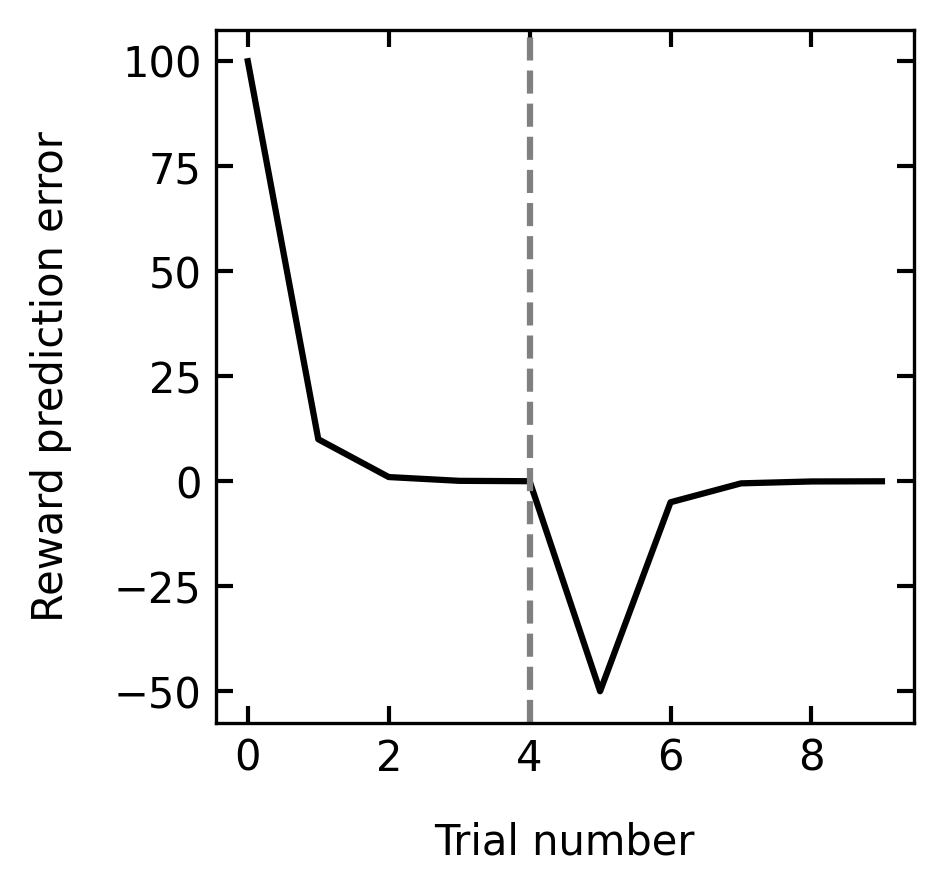
\includegraphics{/home/nicoluarte/uni/PHD/UI/figure1.png}
\caption{Figure shows a series of 10 trials, where from trial 0-4 the
true reward value is 100, and for the remaining trial its 50. A very
basic agent was simulated to update its estimates based on the reward
prediction error. Initial estimates were set at 0. Notice how during
trial 0-4 reward prediction errors are positive and decrease to 0,
because the reward obtained was, initially, greater than the estimate.
In contrast, in trial 5, when reward changes to 50, the error becomes
negative because the estimate was near 100\label{rpe}}
\end{figure}

\begin{figure}
\centering
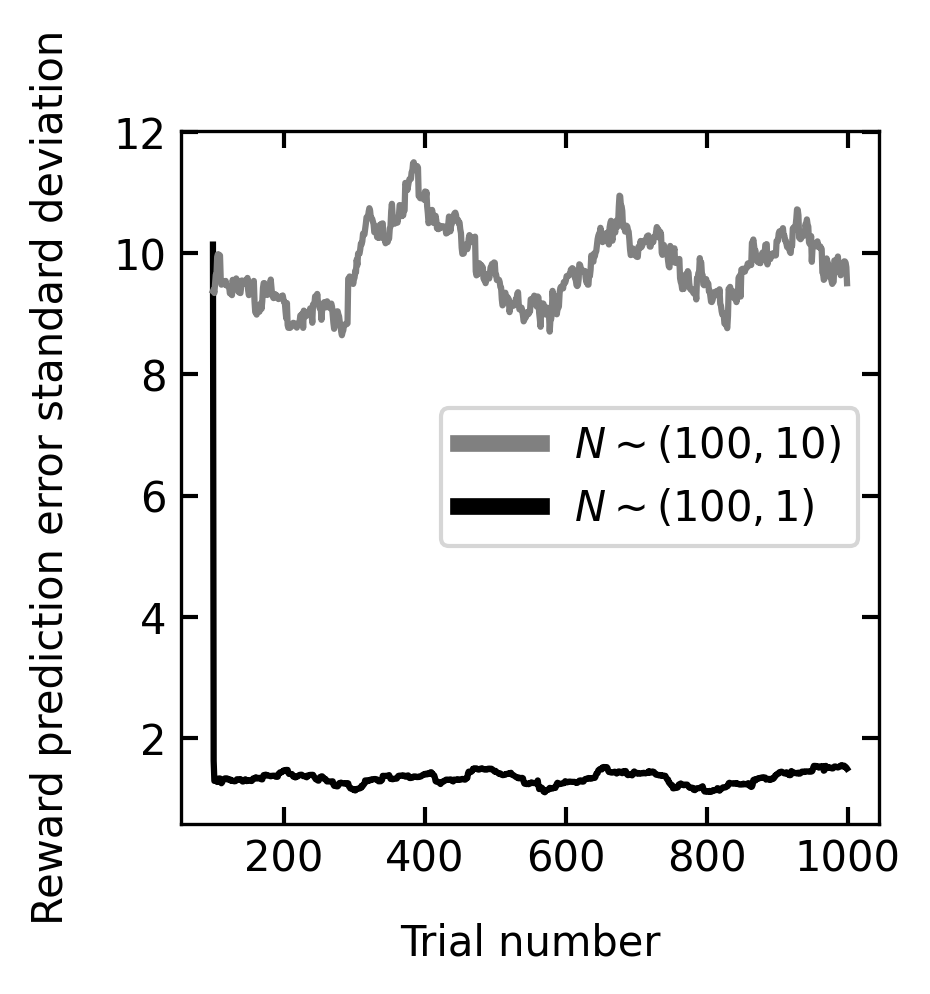
\includegraphics{/home/nicoluarte/uni/PHD/UI/figure2.png}
\caption{Simulated agent learning under two environments, (1) in gray,
rewards are sampled from a normal distribution with mean = 100 and
standard deviation = 10, (2) in black, mean = 100 and standard deviation
= 1. Black and gray lines represent the reward prediction error rolling
standard deviation over 100 trials. Notice how, over the trials, this
`signal' approximates to the underlying uncertainty of the distribution
(using the standard deviation as measure of uncertainty).
\label{uncertainty}}
\end{figure}

\begin{figure}
\centering
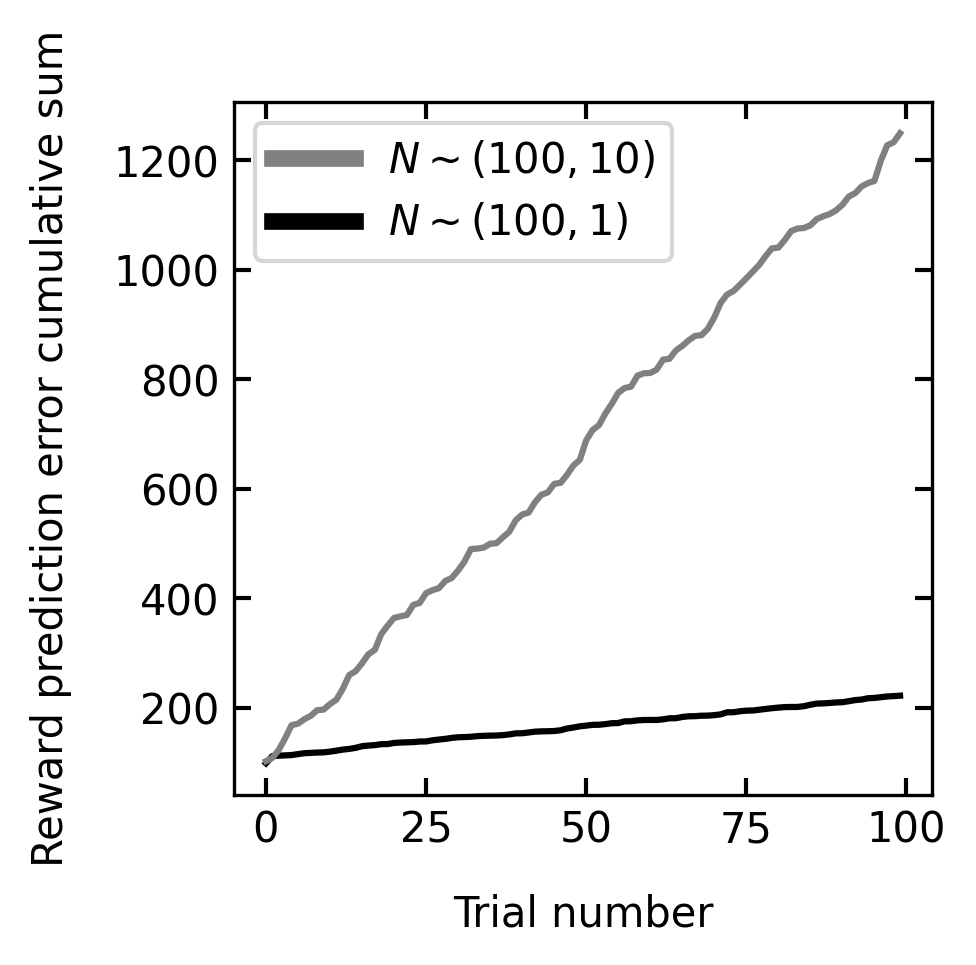
\includegraphics{/home/nicoluarte/uni/PHD/UI/figure3.png}
\caption{Simulated agent learning under two environments, (1) in gray,
rewards are sampled from a normal distribution with mean = 100 and
standard deviation = 10, (2) in black, mean = 100 and standard deviation
= 1. Agent in the environment with higher reward variability (gray), has
a prediction error that varies proportional to reward standard
deviation, so its cumulative sum describes a steeper line than the agent
drawing from lower standard deviation rewards. Note that under ideal
situations, both agents will converge to the reward true value, however,
in the more uncertain environment this will happen at a slower pace.
\label{uncertainty_error}}
\end{figure}

\newpage

\begin{figure}
\centering
\includegraphics{/home/nicoluarte/graphabs.png}
\caption{Graphical abstract}
\end{figure}

\newpage

\hypertarget{references}{%
\section{References}\label{references}}

\hypertarget{refs}{}
\begin{CSLReferences}{1}{0}
\leavevmode\hypertarget{ref-FCVQ7SB6}{}%
Amlung, M., Petker, T., Jackson, J., Balodis, I., \& MacKillop, J.
(2016). Steep discounting of delayed monetary and food rewards in
obesity: a meta-analysis. \emph{Psychological Medicine}, \emph{46}(11),
2423--2434. \url{https://doi.org/10.1017/S0033291716000866}

\leavevmode\hypertarget{ref-LJVQFQ6K}{}%
Anand, B. K., \& Brobeck, J. R. (1951). Localization of a {``Feeding
Center''} in the Hypothalamus of the Rat. \emph{Experimental Biology and
Medicine}, \emph{77}(2), 323--325.
\url{https://doi.org/10.3181/00379727-77-18766}

\leavevmode\hypertarget{ref-UQ9I8YFE}{}%
Ang, Y. N., Wee, B. S., Poh, B. K., \& Ismail, M. N. (2013).
Multifactorial Influences of Childhood Obesity. \emph{Current Obesity
Reports}, \emph{2}(1), 10--22.
\url{https://doi.org/10.1007/s13679-012-0042-7}

\leavevmode\hypertarget{ref-C6Z374UG}{}%
Anselme, P., \& Güntürkün, O. (2019). How foraging works: Uncertainty
magnifies food-seeking motivation. \emph{Behavioral and Brain Sciences},
\emph{42}, e35. \url{https://doi.org/10.1017/S0140525X18000948}

\leavevmode\hypertarget{ref-S8CHV5KG}{}%
Anselme, P., Robinson, M. J. F., \& Berridge, K. C. (2013). Reward
uncertainty enhances incentive salience attribution as sign-tracking.
\emph{Behavioural Brain Research}, \emph{238}, 53--61.
\url{https://doi.org/10.1016/j.bbr.2012.10.006}

\leavevmode\hypertarget{ref-QFWKWDA5}{}%
Ardianto, C., Yonemochi, N., Yamamoto, S., Yang, L., Takenoya, F.,
Shioda, S., Nagase, H., Ikeda, H., \& Kamei, J. (2016). Opioid systems
in the lateral hypothalamus regulate feeding behavior through orexin and
GABA neurons. \emph{Neuroscience}, \emph{320}, 183--193.
\url{https://doi.org/10.1016/j.neuroscience.2016.02.002}

\leavevmode\hypertarget{ref-9MIJEAWP}{}%
Aston-Jones, G., Smith, R. J., Sartor, G. C., Moorman, D. E., Massi, L.,
Tahsili-Fahadan, P., \& Richardson, K. A. (2010). Lateral hypothalamic
orexin/hypocretin neurons: A role in reward-seeking and addiction.
\emph{Brain Research}, \emph{1314}, 74--90.
\url{https://doi.org/10.1016/j.brainres.2009.09.106}

\leavevmode\hypertarget{ref-NXA58KQ4}{}%
Auer, P., Cesa-Bianchi, N., \& Fischer, P. (2002). Finite-time Analysis
of the Multiarmed Bandit Problem. \emph{Machine Learning},
\emph{47}(2/3), 235--256. \url{https://doi.org/10.1023/A:1013689704352}

\leavevmode\hypertarget{ref-XIJMRM6S}{}%
Baimel, C., Lau, B. K., Qiao, M., \& Borgland, S. L. (2017).
Projection-Target-Defined Effects of Orexin and Dynorphin on VTA
Dopamine Neurons. \emph{Cell Reports}, \emph{18}(6), 1346--1355.
\url{https://doi.org/10.1016/j.celrep.2017.01.030}

\leavevmode\hypertarget{ref-6JBBK7KQ}{}%
Balleine, B. W., Delgado, M. R., \& Hikosaka, O. (2007). The Role of the
Dorsal Striatum in Reward and Decision-Making. \emph{Journal of
Neuroscience}, \emph{27}(31), 8161--8165.
\url{https://doi.org/10.1523/JNEUROSCI.1554-07.2007}

\leavevmode\hypertarget{ref-X8KX96JF}{}%
Barrett, C. B. (2010). Measuring Food Insecurity. \emph{Science},
\emph{327}(5967), 825--828.
\url{https://doi.org/10.1126/science.1182768}

\leavevmode\hypertarget{ref-9XCDNBAM}{}%
Bartumeus, F., Campos, D., Ryu, W. S., Lloret-Cabot, R., Méndez, V., \&
Catalan, J. (2016). Foraging success under uncertainty: search tradeoffs
and optimal space use. \emph{Ecology Letters}, \emph{19}(11),
1299--1313. \url{https://doi.org/10.1111/ele.12660}

\leavevmode\hypertarget{ref-BGNECK7I}{}%
Bayard, S., Abril, B., Yu, H., Scholz, S., Carlander, B., \&
Dauvilliers, Y. (2011). Decision Making in Narcolepsy with Cataplexy.
\emph{Sleep}, \emph{34}(1), 99--104.
\url{https://doi.org/10.1093/sleep/34.1.99}

\leavevmode\hypertarget{ref-ZHGB75KH}{}%
Bayer, H. M., \& Glimcher, P. W. (2005). Midbrain Dopamine Neurons
Encode a Quantitative Reward Prediction Error Signal. \emph{Neuron},
\emph{47}(1), 129--141.
\url{https://doi.org/10.1016/j.neuron.2005.05.020}

\leavevmode\hypertarget{ref-LLLWQCZE}{}%
Bednekoff, P. A., \& Houston, A. I. (1994). Avian daily foraging
patterns: Effects of digestive constraints and variability.
\emph{Evolutionary Ecology}, \emph{8}(1), 36--52.
\url{https://doi.org/10.1007/BF01237664}

\leavevmode\hypertarget{ref-BHR2NAEI}{}%
Behrens, T. E. J., Woolrich, M. W., Walton, M. E., \& Rushworth, M. F.
S. (2007). Learning the value of information in an uncertain world.
\emph{Nature Neuroscience}, \emph{10}(9), 1214--1221.
\url{https://doi.org/10.1038/nn1954}

\leavevmode\hypertarget{ref-8QS2B4AF}{}%
Best, J. R., Theim, K. R., Gredysa, D. M., Stein, R. I., Welch, R. R.,
Saelens, B. E., Perri, M. G., Schechtman, K. B., Epstein, L. H., \&
Wilfley, D. E. (2012). Behavioral economic predictors of overweight
children's weight loss. \emph{Journal of Consulting and Clinical
Psychology}, \emph{80}(6), 1086--1096.
\url{https://doi.org/10.1037/a0029827}

\leavevmode\hypertarget{ref-BFYKZGMM}{}%
Bhadoria, A., Sahoo, K., Sahoo, B., Choudhury, A., Sufi, N., \& Kumar,
R. (2015). Childhood obesity: Causes and consequences. \emph{Journal of
Family Medicine and Primary Care}, \emph{4}(2), 187.
\url{https://doi.org/10.4103/2249-4863.154628}

\leavevmode\hypertarget{ref-AFIWCGVS}{}%
Blanco, N. J., \& Sloutsky, V. (2019). \emph{Systematic Exploration and
Uncertainty Dominate Young Children's Choices}. PsyArXiv.
\url{https://osf.io/72sfx}

\leavevmode\hypertarget{ref-PN23NXIS}{}%
Bordier, C., Klein, S., Le Conte, Y., Barron, A. B., \& Alaux, C.
(2018). Stress decreases pollen foraging performance in honeybees.
\emph{The Journal of Experimental Biology}, \emph{221}(4), jeb171470.
\url{https://doi.org/10.1242/jeb.171470}

\leavevmode\hypertarget{ref-VTI2FVJG}{}%
Brunstrom, J. M., \& Cheon, B. K. (2018). Do humans still forage in an
obesogenic environment? Mechanisms and implications for weight
maintenance. \emph{Physiology \& Behavior}, \emph{193}, 261--267.
\url{https://doi.org/10.1016/j.physbeh.2018.02.038}

\leavevmode\hypertarget{ref-IQWZPMP7}{}%
Burdakov, D. (2019). Reactive and predictive homeostasis: Roles of
orexin/hypocretin neurons. \emph{Neuropharmacology}, \emph{154}, 61--67.
\url{https://doi.org/10.1016/j.neuropharm.2018.10.024}

\leavevmode\hypertarget{ref-9I3RBWWB}{}%
Buyukdere, Y., Gulec, A., \& Akyol, A. (2019). Cafeteria diet increased
adiposity in comparison to high fat diet in young male rats.
\emph{PeerJ}, \emph{7}, e6656. \url{https://doi.org/10.7717/peerj.6656}

\leavevmode\hypertarget{ref-GDQBDJJ2}{}%
Carlier, N., Marshe, V. S., Cmorejova, J., Davis, C., \& Müller, D. J.
(2015). Genetic Similarities between Compulsive Overeating and Addiction
Phenotypes: A Case for {``Food Addiction?''} \emph{Current Psychiatry
Reports}, \emph{17}(12), 96.
\url{https://doi.org/10.1007/s11920-015-0634-5}

\leavevmode\hypertarget{ref-8FIHXB6G}{}%
Chakroun, K., Mathar, D., Wiehler, A., Ganzer, F., \& Peters, J. (2020).
Dopaminergic modulation of the exploration/exploitation trade-off in
human decision-making. \emph{eLife}, \emph{9}, e51260.
\url{https://doi.org/10.7554/eLife.51260}

\leavevmode\hypertarget{ref-ESYGCSLH}{}%
Charnov, E. L. (1976). Optimal foraging, the marginal value theorem.
\emph{Theoretical Population Biology}, \emph{9}(2), 129--136.
\url{https://doi.org/10.1016/0040-5809(76)90040-X}

\leavevmode\hypertarget{ref-P3MLPUGY}{}%
Collins, L., Young, D. B., Davies, K., \& Pearce, J. M. (1983). The
Influence of Partial Reinforcement on Serial Autoshaping with Pigeons.
\emph{The Quarterly Journal of Experimental Psychology Section B},
\emph{35}(4b), 275--290. \url{https://doi.org/10.1080/14640748308400893}

\leavevmode\hypertarget{ref-6ZEIWIGL}{}%
Colombo, M. (2014). Deep and beautiful. The reward prediction error
hypothesis of dopamine. \emph{Studies in History and Philosophy of
Science Part C: Studies in History and Philosophy of Biological and
Biomedical Sciences}, \emph{45}, 57--67.
\url{https://doi.org/10.1016/j.shpsc.2013.10.006}

\leavevmode\hypertarget{ref-YI6J6Y7I}{}%
Craft, B. B. (2016). Risk-sensitive foraging: changes in choice due to
reward quality and delay. \emph{Animal Behaviour}, \emph{111}, 41--47.
\url{https://doi.org/10.1016/j.anbehav.2015.09.030}

\leavevmode\hypertarget{ref-3GQMEPEH}{}%
Cuthill, I. C. (2000). Body mass regulation in response to changes in
feeding predictability and overnight energy expenditure.
\emph{Behavioral Ecology}, \emph{11}(2), 189--195.
\url{https://doi.org/10.1093/beheco/11.2.189}

\leavevmode\hypertarget{ref-8TKQDEML}{}%
D'Ardenne, K., McClure, S. M., Nystrom, L. E., \& Cohen, J. D. (2008).
BOLD Responses Reflecting Dopaminergic Signals in the Human Ventral
Tegmental Area. \emph{Science}, \emph{319}(5867), 1264--1267.
\url{https://doi.org/10.1126/science.1150605}

\leavevmode\hypertarget{ref-9YRMQU6H}{}%
da Matta, A., Gonçalves, F. L., \& Bizarro, L. (2012). Delay
discounting: Concepts and measures. \emph{Psychology \& Neuroscience},
\emph{5}(2), 135--146. \url{https://doi.org/10.3922/j.psns.2012.2.03}

\leavevmode\hypertarget{ref-D6LH64XI}{}%
Dao, M. C., Messer, E., Conigliaro, T., Sakaida, K., Ouellette, A. F.,
Himaras, V., Thiron, S., \& Roberts, S. B. (2019). Different and
Unequal: A Qualitative Evaluation of Salient Factors Influencing Energy
Intake in Adults with Overweight and Obesity. \emph{Nutrients},
\emph{11}(6), 1365. \url{https://doi.org/10.3390/nu11061365}

\leavevmode\hypertarget{ref-67T2WUWD}{}%
Davis, C., Levitan, R. D., Muglia, P., Bewell, C., \& Kennedy, J. L.
(2004). Decision-Making Deficits and Overeating: A Risk Model for
Obesity. \emph{Obesity Research}, \emph{12}(6), 929--935.
\url{https://doi.org/10.1038/oby.2004.113}

\leavevmode\hypertarget{ref-9SRBHI4W}{}%
Davis, J. F., Choi, D. L., \& Benoit, S. C. (2010). Insulin, leptin and
reward. \emph{Trends in Endocrinology \& Metabolism}, \emph{21}(2),
68--74. \url{https://doi.org/10.1016/j.tem.2009.08.004}

\leavevmode\hypertarget{ref-JZJAAAYD}{}%
Daw, N. D., Kakade, S., \& Dayan, P. (2002). Opponent interactions
between serotonin and dopamine. \emph{Neural Networks}, \emph{15}(4-6),
603--616. \url{https://doi.org/10.1016/S0893-6080(02)00052-7}

\leavevmode\hypertarget{ref-WLQDZ5HW}{}%
de Berker, A. O., Rutledge, R. B., Mathys, C., Marshall, L., Cross, G.
F., Dolan, R. J., \& Bestmann, S. (2016). Computations of uncertainty
mediate acute stress responses in humans. \emph{Nature Communications},
\emph{7}(1), 10996. \url{https://doi.org/10.1038/ncomms10996}

\leavevmode\hypertarget{ref-AF2655I2}{}%
De Groot, K., \& Thurik, R. (2018). Disentangling Risk and Uncertainty:
When Risk-Taking Measures Are Not About Risk. \emph{Frontiers in
Psychology}, \emph{9}, 2194.
\url{https://doi.org/10.3389/fpsyg.2018.02194}

\leavevmode\hypertarget{ref-V8LPCV6E}{}%
Delgado, J. M. R., \& Anand, B. K. (1952). Increase of Food Intake
Induced by Electrical Stimulation of the Lateral Hypothalamus.
\emph{American Journal of Physiology-Legacy Content}, \emph{172}(1),
162--168. \url{https://doi.org/10.1152/ajplegacy.1952.172.1.162}

\leavevmode\hypertarget{ref-CMAIA6R7}{}%
Diederen, K. M. J., \& Schultz, W. (2015). Scaling prediction errors to
reward variability benefits error-driven learning in humans.
\emph{Journal of Neurophysiology}, \emph{114}(3), 1628--1640.
\url{https://doi.org/10.1152/jn.00483.2015}

\leavevmode\hypertarget{ref-2HED3PSJ}{}%
DiLeone, R. J., Georgescu, D., \& Nestler, E. J. (2003). Lateral
hypothalamic neuropeptides in reward and drug addiction. \emph{Life
Sciences}, \emph{73}(6), 759--768.
\url{https://doi.org/10.1016/S0024-3205(03)00408-9}

\leavevmode\hypertarget{ref-JPZD7WDQ}{}%
Enomoto, K., Matsumoto, N., Nakai, S., Satoh, T., Sato, T. K., Ueda, Y.,
Inokawa, H., Haruno, M., \& Kimura, M. (2011). Dopamine neurons learn to
encode the long-term value of multiple future rewards. \emph{Proceedings
of the National Academy of Sciences}, \emph{108}(37), 15462--15467.
\url{https://doi.org/10.1073/pnas.1014457108}

\leavevmode\hypertarget{ref-TLRSYNN6}{}%
Epstein, L. H., Jankowiak, N., Fletcher, K. D., Carr, K. A., Nederkoorn,
C., Raynor, H. A., \& Finkelstein, E. (2014). Women who are motivated to
eat and discount the future are more obese: BMI and Reinforcement
Pathology. \emph{Obesity}, \emph{22}(6), 1394--1399.
\url{https://doi.org/10.1002/oby.20661}

\leavevmode\hypertarget{ref-R775Y2Q6}{}%
Eshel, N., Tian, J., Bukwich, M., \& Uchida, N. (2016). Dopamine neurons
share common response function for reward prediction error. \emph{Nature
Neuroscience}, \emph{19}(3), 479--486.
\url{https://doi.org/10.1038/nn.4239}

\leavevmode\hypertarget{ref-89DIP32B}{}%
Even-Dar, E., \& Mansour, Y. (2001). Learning Rates for Q-Learning. In
D. Helmbold \& B. Williamson (Eds.), \emph{Computational Learning
Theory} (Vol. 2111, pp. 589--604). Springer Berlin Heidelberg.
\url{http://link.springer.com/10.1007/3-540-44581-1_39}

\leavevmode\hypertarget{ref-4PLXQQT9}{}%
Fadel, J., \& Deutch, A. Y. (2002). Anatomical substrates of
orexin--dopamine interactions: lateral hypothalamic projections to the
ventral tegmental area. \emph{Neuroscience}, \emph{111}(2), 379--387.
\url{https://doi.org/10.1016/S0306-4522(02)00017-9}

\leavevmode\hypertarget{ref-Q3Q977MQ}{}%
Faraji, M., Preuschoff, K., \& Gerstner, W. (2017). Balancing New
Against Old Information: The Role of Surprise in Learning.
\emph{arXiv:1606.05642 {[}cs, q-Bio, Stat{]}}.
\url{http://arxiv.org/abs/1606.05642}

\leavevmode\hypertarget{ref-WS9KYIYG}{}%
Fawcett, T. W., Fallenstein, B., Higginson, A. D., Houston, A. I.,
Mallpress, D. E. W., Trimmer, P. C., \& McNamara, J. M. (2014). The
evolution of decision rules in complex environments. \emph{Trends in
Cognitive Sciences}, \emph{18}(3), 153--161.
\url{https://doi.org/10.1016/j.tics.2013.12.012}

\leavevmode\hypertarget{ref-NBA5EBE8}{}%
Fazzino, T. L., Rohde, K., \& Sullivan, D. K. (2019). Hyper‐Palatable
Foods: Development of a Quantitative Definition and Application to the
US Food System Database. \emph{Obesity}, \emph{27}(11), 1761--1768.
\url{https://doi.org/10.1002/oby.22639}

\leavevmode\hypertarget{ref-B3IPWFXL}{}%
Ferretti, A., Maggini, I., Lupi, S., Cardinale, M., \& Fusani, L.
(2019). The amount of available food affects diurnal locomotor activity
in migratory songbirds during stopover. \emph{Scientific Reports},
\emph{9}(1), 19027. \url{https://doi.org/10.1038/s41598-019-55404-3}

\leavevmode\hypertarget{ref-VWAZILDA}{}%
Filbey, F. M., Myers, U. S., \& DeWitt, S. (2012). Reward circuit
function in high BMI individuals with compulsive overeating:
Similarities with addiction. \emph{NeuroImage}, \emph{63}(4),
1800--1806. \url{https://doi.org/10.1016/j.neuroimage.2012.08.073}

\leavevmode\hypertarget{ref-X6X8T8QT}{}%
Filipowicz, A. L., Glaze, C. M., Kable, J. W., \& Gold, J. I. (2020).
Pupil diameter encodes the idiosyncratic, cognitive complexity of belief
updating. \emph{eLife}, \emph{9}, e57872.
\url{https://doi.org/10.7554/eLife.57872}

\leavevmode\hypertarget{ref-AR2TQB84}{}%
Fiorillo, C. D. (2003). Discrete Coding of Reward Probability and
Uncertainty by Dopamine Neurons. \emph{Science}, \emph{299}(5614),
1898--1902. \url{https://doi.org/10.1126/science.1077349}

\leavevmode\hypertarget{ref-UTKKIKVA}{}%
Fitzpatrick, S., Gilbert, S., \& Serpell, L. (2013). Systematic Review:
Are Overweight and Obese Individuals Impaired on Behavioural Tasks of
Executive Functioning? \emph{Neuropsychology Review}, \emph{23}(2),
138--156. \url{https://doi.org/10.1007/s11065-013-9224-7}

\leavevmode\hypertarget{ref-BDFISDRS}{}%
Flagel, S. B. (2014). Sign-Tracking. In I. P. Stolerman \& L. H. Price
(Eds.), \emph{Encyclopedia of Psychopharmacology} (pp. 1--7). Springer
Berlin Heidelberg.
\url{http://link.springer.com/10.1007/978-3-642-27772-6_7020-1}

\leavevmode\hypertarget{ref-CFC7DN65}{}%
Fokidis, H. B., des Roziers, M. B., Sparr, R., Rogowski, C., Sweazea,
K., \& Deviche, P. (2012). Unpredictable food availability induces
metabolic and hormonal changes independent of food intake in a sedentary
songbird. \emph{Journal of Experimental Biology}, \emph{215}(16),
2920--2930. \url{https://doi.org/10.1242/jeb.071043}

\leavevmode\hypertarget{ref-NL4XYLRH}{}%
Forkman, B. A. (1993). The Effect of Uncertainty On the Food Intake of
the Mongolian Gerbil. \emph{Behaviour}, \emph{124}(3-4), 197--206.
\url{https://doi.org/10.1163/156853993X00579}

\leavevmode\hypertarget{ref-V9CIKRBE}{}%
Friston, K. (2009). The free-energy principle: a rough guide to the
brain? \emph{Trends in Cognitive Sciences}, \emph{13}(7), 293--301.
\url{https://doi.org/10.1016/j.tics.2009.04.005}

\leavevmode\hypertarget{ref-4JUZW55S}{}%
García-García, I., Horstmann, A., Jurado, M. A., Garolera, M., Chaudhry,
S. J., Margulies, D. S., Villringer, A., \& Neumann, J. (2014). Reward
processing in obesity, substance addiction and non-substance addiction:
Obesity, addictions and reward. \emph{Obesity Reviews}, \emph{15}(11),
853--869. \url{https://doi.org/10.1111/obr.12221}

\leavevmode\hypertarget{ref-S3LMSWG5}{}%
Geisler, S., Derst, C., Veh, R. W., \& Zahm, D. S. (2007). Glutamatergic
Afferents of the Ventral Tegmental Area in the Rat. \emph{Journal of
Neuroscience}, \emph{27}(21), 5730--5743.
\url{https://doi.org/10.1523/JNEUROSCI.0012-07.2007}

\leavevmode\hypertarget{ref-SC7QH8NN}{}%
Geisler, Stefanie, \& Zahm, D. S. (2005). Afferents of the ventral
tegmental area in the rat-anatomical substratum for integrative
functions. \emph{The Journal of Comparative Neurology}, \emph{490}(3),
270--294. \url{https://doi.org/10.1002/cne.20668}

\leavevmode\hypertarget{ref-LFIY67XG}{}%
Gershman, S. J. (2018). Deconstructing the human algorithms for
exploration. \emph{Cognition}, \emph{173}, 34--42.
\url{https://doi.org/10.1016/j.cognition.2017.12.014}

\leavevmode\hypertarget{ref-SZZJ3VQF}{}%
Gershman, S. J. (2017). Dopamine, Inference, and Uncertainty.
\emph{Neural Computation}, \emph{29}(12), 3311--3326.
\url{https://doi.org/10.1162/neco_a_01023}

\leavevmode\hypertarget{ref-R3TZXYBW}{}%
Glimcher, P. W. (2011). Understanding dopamine and reinforcement
learning: The dopamine reward prediction error hypothesis.
\emph{Proceedings of the National Academy of Sciences},
\emph{108}(Supplement\_3), 15647--15654.
\url{https://doi.org/10.1073/pnas.1014269108}

\leavevmode\hypertarget{ref-J7XQF8LY}{}%
Hafenbrädl, S., Waeger, D., Marewski, J. N., \& Gigerenzer, G. (2016).
Applied Decision Making With Fast-and-Frugal Heuristics. \emph{Journal
of Applied Research in Memory and Cognition}, \emph{5}(2), 215--231.
\url{https://doi.org/10.1016/j.jarmac.2016.04.011}

\leavevmode\hypertarget{ref-C6PMZNGR}{}%
Hariri, N., \& Thibault, L. (2010). High-fat diet-induced obesity in
animal models. \emph{Nutrition Research Reviews}, \emph{23}(2),
270--299. \url{https://doi.org/10.1017/S0954422410000168}

\leavevmode\hypertarget{ref-TUU47UNG}{}%
Harris, G. C., \& Aston-Jones, G. (2006). Arousal and reward: a
dichotomy in orexin function. \emph{Trends in Neurosciences},
\emph{29}(10), 571--577.
\url{https://doi.org/10.1016/j.tins.2006.08.002}

\leavevmode\hypertarget{ref-S6TNU7XM}{}%
Harris, G. C., Wimmer, M., \& Aston-Jones, G. (2005). A role for lateral
hypothalamic orexin neurons in reward seeking. \emph{Nature},
\emph{437}(7058), 556--559. \url{https://doi.org/10.1038/nature04071}

\leavevmode\hypertarget{ref-G83L8BXA}{}%
Harris, T. R., Chapman, C. A., \& Monfort, S. L. (2010). Small
folivorous primate groups exhibit behavioral and physiological effects
of food scarcity. \emph{Behavioral Ecology}, \emph{21}(1), 46--56.
\url{https://doi.org/10.1093/beheco/arp150}

\leavevmode\hypertarget{ref-DAKDZEVY}{}%
Haruno, M., \& Kawato, M. (2006). Different neural correlates of reward
expectation and reward expectation error in the putamen and caudate
nucleus during stimulus-action-reward association learning.
\emph{Journal of Neurophysiology}, \emph{95}(2), 948--959.
\url{https://doi.org/10.1152/jn.00382.2005}

\leavevmode\hypertarget{ref-J37T9F5T}{}%
Higgs, S. (2016). Cognitive processing of food rewards. \emph{Appetite},
\emph{104}, 10--17. \url{https://doi.org/10.1016/j.appet.2015.10.003}

\leavevmode\hypertarget{ref-A5N6NMAB}{}%
Hills, T. T., Kalff, C., \& Wiener, J. M. (2013). Adaptive Lévy
Processes and Area-Restricted Search in Human Foraging. \emph{PLoS ONE},
\emph{8}(4), e60488. \url{https://doi.org/10.1371/journal.pone.0060488}

\leavevmode\hypertarget{ref-67GSY6VY}{}%
Horstmann, A., Fenske, W. K., \& Hankir, M. K. (2015). Argument for a
non-linear relationship between severity of human obesity and
dopaminergic tone: Relationship between obesity and dopaminergic tone.
\emph{Obesity Reviews}, \emph{16}(10), 821--830.
\url{https://doi.org/10.1111/obr.12303}

\leavevmode\hypertarget{ref-ZRTDBMRA}{}%
Huettel, S. A. (2005). Decisions under Uncertainty: Probabilistic
Context Influences Activation of Prefrontal and Parietal Cortices.
\emph{Journal of Neuroscience}, \emph{25}(13), 3304--3311.
\url{https://doi.org/10.1523/JNEUROSCI.5070-04.2005}

\leavevmode\hypertarget{ref-M5RXPXSZ}{}%
Humphries, N. E., \& Sims, D. W. (2014). Optimal foraging strategies:
Lévy walks balance searching and patch exploitation under a very broad
range of conditions. \emph{Journal of Theoretical Biology}, \emph{358},
179--193. \url{https://doi.org/10.1016/j.jtbi.2014.05.032}

\leavevmode\hypertarget{ref-JGKMEKV6}{}%
Huys, Q. J., Pizzagalli, D. A., Bogdan, R., \& Dayan, P. (2013). Mapping
anhedonia onto reinforcement learning: a behavioural meta-analysis.
\emph{Biology of Mood \& Anxiety Disorders}, \emph{3}(1), 12.
\url{https://doi.org/10.1186/2045-5380-3-12}

\leavevmode\hypertarget{ref-2ZT7CAFB}{}%
Jennings, J. H., Rizzi, G., Stamatakis, A. M., Ung, R. L., \& Stuber, G.
D. (2013). The Inhibitory Circuit Architecture of the Lateral
Hypothalamus Orchestrates Feeding. \emph{Science}, \emph{341}(6153),
1517--1521. \url{https://doi.org/10.1126/science.1241812}

\leavevmode\hypertarget{ref-LIRXSMKQ}{}%
Jepma, M., Murphy, P. R., Nassar, M. R., Rangel-Gomez, M., Meeter, M.,
\& Nieuwenhuis, S. (2016). Catecholaminergic Regulation of Learning Rate
in a Dynamic Environment. \emph{PLOS Computational Biology},
\emph{12}(10), e1005171.
\url{https://doi.org/10.1371/journal.pcbi.1005171}

\leavevmode\hypertarget{ref-KA4Y29AG}{}%
Kane, G. A., Vazey, E. M., Wilson, R. C., Shenhav, A., Daw, N. D.,
Aston-Jones, G., \& Cohen, J. D. (2017). Increased locus coeruleus tonic
activity causes disengagement from a patch-foraging task.
\emph{Cognitive, Affective, \& Behavioral Neuroscience}, \emph{17}(6),
1073--1083. \url{https://doi.org/10.3758/s13415-017-0531-y}

\leavevmode\hypertarget{ref-E6MZ8HIA}{}%
Keiflin, R., Pribut, H. J., Shah, N. B., \& Janak, P. H. (2019). Ventral
Tegmental Dopamine Neurons Participate in Reward Identity Predictions.
\emph{Current Biology}, \emph{29}(1), 93--103.e3.
\url{https://doi.org/10.1016/j.cub.2018.11.050}

\leavevmode\hypertarget{ref-P8YAF6NZ}{}%
Kempadoo, K. A., Tourino, C., Cho, S. L., Magnani, F., Leinninger,
G.-M., Stuber, G. D., Zhang, F., Myers, M. G., Deisseroth, K., de Lecea,
L., \& Bonci, A. (2013). Hypothalamic Neurotensin Projections Promote
Reward by Enhancing Glutamate Transmission in the VTA. \emph{Journal of
Neuroscience}, \emph{33}(18), 7618--7626.
\url{https://doi.org/10.1523/JNEUROSCI.2588-12.2013}

\leavevmode\hypertarget{ref-TPGJBDDD}{}%
Kotz, C. M., Teske, J. A., Levine, J. A., \& Wang, C. (2002). Feeding
and activity induced by orexin A in the lateral hypothalamus in rats.
\emph{Regulatory Peptides}, \emph{104}(1-3), 27--32.
\url{https://doi.org/10.1016/S0167-0115(01)00346-9}

\leavevmode\hypertarget{ref-GU4KJGAS}{}%
Kroemer, N. B., \& Small, D. M. (2016). Fuel not fun: Reinterpreting
attenuated brain responses to reward in obesity. \emph{Physiology \&
Behavior}, \emph{162}, 37--45.
\url{https://doi.org/10.1016/j.physbeh.2016.04.020}

\leavevmode\hypertarget{ref-PE46B3Z8}{}%
Kube, J., Mathar, D., Horstmann, A., Kotz, S. A., Villringer, A., \&
Neumann, J. (2018). Altered monetary loss processing and
reinforcement-based learning in individuals with obesity. \emph{Brain
Imaging and Behavior}, \emph{12}(5), 1431--1449.
\url{https://doi.org/10.1007/s11682-017-9786-8}

\leavevmode\hypertarget{ref-EBJDV6NP}{}%
Leigh, S.-J., Kendig, M. D., \& Morris, M. J. (2019). Palatable
Western-style Cafeteria Diet as a Reliable Method for Modeling
Diet-induced Obesity in Rodents. \emph{Journal of Visualized
Experiments}, \emph{153}, 60262. \url{https://doi.org/10.3791/60262}

\leavevmode\hypertarget{ref-GDVXZGJY}{}%
Leinninger, G. M., Jo, Y.-H., Leshan, R. L., Louis, G. W., Yang, H.,
Barrera, J. G., Wilson, H., Opland, D. M., Faouzi, M. A., Gong, Y.,
Jones, J. C., Rhodes, C. J., Chua, S., Diano, S., Horvath, T. L.,
Seeley, R. J., Becker, J. B., Münzberg, H., \& Myers, M. G. (2009).
Leptin Acts via Leptin Receptor-Expressing Lateral Hypothalamic Neurons
to Modulate the Mesolimbic Dopamine System and Suppress Feeding.
\emph{Cell Metabolism}, \emph{10}(2), 89--98.
\url{https://doi.org/10.1016/j.cmet.2009.06.011}

\leavevmode\hypertarget{ref-8RIQXAVT}{}%
Lohmus, M., Sundstrom, L. F., \& Moore, F. R. (2006). Non-invasive
corticosterone treatment changes foraging intensity in red-eyed vireos
Vireo olivaceus. \emph{Journal of Avian Biology}, \emph{37}(5),
523--526. \url{https://doi.org/10.1111/j.0908-8857.2006.03733.x}

\leavevmode\hypertarget{ref-S8GZWPNK}{}%
Louie, K., Khaw, M. W., \& Glimcher, P. W. (2013). Normalization is a
general neural mechanism for context-dependent decision making.
\emph{Proceedings of the National Academy of Sciences}, \emph{110}(15),
6139--6144. \url{https://doi.org/10.1073/pnas.1217854110}

\leavevmode\hypertarget{ref-8XA5RHVI}{}%
Macleod, R., Barnett, P., Clark, J. A., \& Cresswell, W. (2005). Body
mass change strategies in blackbirds Turdus merula: the
starvation-predation risk trade-off. \emph{Journal of Animal Ecology},
\emph{74}(2), 292--302.
\url{https://doi.org/10.1111/j.1365-2656.2005.00923.x}

\leavevmode\hypertarget{ref-YMQYAEQ8}{}%
Mahmoudi, M., Maleki-Roveshti, M., Karimi-Haghighi, S., \& Haghparast,
A. (2020). Chemical stimulation of the lateral hypothalamus induced
seeking behaviors in rats: Involvement of orexin receptors in the
ventral tegmental area. \emph{European Journal of Pharmacology},
\emph{886}, 173433. \url{https://doi.org/10.1016/j.ejphar.2020.173433}

\leavevmode\hypertarget{ref-MW2YHV9D}{}%
Margules, D. L., \& Olds, J. (1962). Identical {``Feeding''} and
{``Rewarding''} Systems in the Lateral Hypothalamus of Rats.
\emph{Science}, \emph{135}(3501), 374--375.
\url{https://doi.org/10.1126/science.135.3501.374}

\leavevmode\hypertarget{ref-ELZ2PYYM}{}%
Mascia, P., Neugebauer, N. M., Brown, J., Bubula, N., Nesbitt, K. M.,
Kennedy, R. T., \& Vezina, P. (2019). Exposure to conditions of
uncertainty promotes the pursuit of amphetamine.
\emph{Neuropsychopharmacology}, \emph{44}(2), 274--280.
\url{https://doi.org/10.1038/s41386-018-0099-4}

\leavevmode\hypertarget{ref-DBGUDZRL}{}%
Mathar, D., Neumann, J., Villringer, A., \& Horstmann, A. (2017).
Failing to learn from negative prediction errors: Obesity is associated
with alterations in a fundamental neural learning mechanism.
\emph{Cortex}, \emph{95}, 222--237.
\url{https://doi.org/10.1016/j.cortex.2017.08.022}

\leavevmode\hypertarget{ref-Q8IHJK68}{}%
Mattar, P., Uribe-Cerda, S., Pezoa, C., Guarnieri, T., Kotz, C. M.,
Teske, J. A., Morselli, E., \& Perez-Leighton, C. (2020). Brain
site-specific regulation of hedonic intake by orexin and DYN peptides:
role of the PVN and obesity. \emph{Nutritional Neuroscience}, 1--10.
\url{https://doi.org/10.1080/1028415X.2020.1840049}

\leavevmode\hypertarget{ref-BUXRNM89}{}%
Mikhael, J. G., \& Bogacz, R. (2016). Learning Reward Uncertainty in the
Basal Ganglia. \emph{PLOS Computational Biology}, \emph{12}(9),
e1005062. \url{https://doi.org/10.1371/journal.pcbi.1005062}

\leavevmode\hypertarget{ref-BW3RY7GD}{}%
Moiron, M., Mathot, K. J., \& Dingemanse, N. J. (2018). To eat and not
be eaten: diurnal mass gain and foraging strategies in wintering great
tits. \emph{Proceedings of the Royal Society B: Biological Sciences},
\emph{285}(1874), 20172868. \url{https://doi.org/10.1098/rspb.2017.2868}

\leavevmode\hypertarget{ref-4LJKTR3N}{}%
Moradi, S., Mirzababaei, A., Dadfarma, A., Rezaei, S., Mohammadi, H.,
Jannat, B., \& Mirzaei, K. (2019). Food insecurity and adult weight
abnormality risk: a systematic review and meta-analysis. \emph{European
Journal of Nutrition}, \emph{58}(1), 45--61.
\url{https://doi.org/10.1007/s00394-018-1819-6}

\leavevmode\hypertarget{ref-XZBUNRIS}{}%
Muranishi, M., Inokawa, H., Yamada, H., Ueda, Y., Matsumoto, N.,
Nakagawa, M., \& Kimura, M. (2011). Inactivation of the putamen
selectively impairs reward history-based action selection.
\emph{Experimental Brain Research}, \emph{209}(2), 235--246.
\url{https://doi.org/10.1007/s00221-011-2545-y}

\leavevmode\hypertarget{ref-C4QSBWHV}{}%
Nambu, T., Sakurai, T., Mizukami, K., Hosoya, Y., Yanagisawa, M., \&
Goto, K. (1999). Distribution of orexin neurons in the adult rat
brain1Published on the World Wide Web on 17 March 1999.1. \emph{Brain
Research}, \emph{827}(1-2), 243--260.
\url{https://doi.org/10.1016/S0006-8993(99)01336-0}

\leavevmode\hypertarget{ref-X596XYG3}{}%
Namdari, A., \& Li, Z. (Steven). (2019). A review of entropy measures
for uncertainty quantification of stochastic processes. \emph{Advances
in Mechanical Engineering}, \emph{11}(6), 168781401985735.
\url{https://doi.org/10.1177/1687814019857350}

\leavevmode\hypertarget{ref-U2GSF8HI}{}%
Nassar, M. R., Rumsey, K. M., Wilson, R. C., Parikh, K., Heasly, B., \&
Gold, J. I. (2012). Rational regulation of learning dynamics by
pupil-linked arousal systems. \emph{Nature Neuroscience}, \emph{15}(7),
1040--1046. \url{https://doi.org/10.1038/nn.3130}

\leavevmode\hypertarget{ref-A9R3LNZJ}{}%
Nettle, D., Andrews, C., \& Bateson, M. (2017). Food insecurity as a
driver of obesity in humans: The insurance hypothesis. \emph{Behavioral
and Brain Sciences}, \emph{40}, e105.
\url{https://doi.org/10.1017/S0140525X16000947}

\leavevmode\hypertarget{ref-HT5LXV4U}{}%
Nieh, Edward~H., Matthews, Gillian~A., Allsop, Stephen~A., Presbrey,
Kara~N., Leppla, Christopher~A., Wichmann, R., Neve, R., Wildes,
Craig~P., \& Tye, Kay~M. (2015). Decoding Neural Circuits that Control
Compulsive Sucrose Seeking. \emph{Cell}, \emph{160}(3), 528--541.
\url{https://doi.org/10.1016/j.cell.2015.01.003}

\leavevmode\hypertarget{ref-GZ3AZ6UU}{}%
Nieh, Edward~H., Vander~Weele, Caitlin~M., Matthews, Gillian~A.,
Presbrey, Kara~N., Wichmann, R., Leppla, Christopher~A., Izadmehr,
Ehsan~M., \& Tye, Kay~M. (2016). Inhibitory Input from the Lateral
Hypothalamus to the Ventral Tegmental Area Disinhibits Dopamine Neurons
and Promotes Behavioral Activation. \emph{Neuron}, \emph{90}(6),
1286--1298. \url{https://doi.org/10.1016/j.neuron.2016.04.035}

\leavevmode\hypertarget{ref-4F2PUL7U}{}%
Nonomura, S., Nishizawa, K., Sakai, Y., Kawaguchi, Y., Kato, S.,
Uchigashima, M., Watanabe, M., Yamanaka, K., Enomoto, K., Chiken, S.,
Sano, H., Soma, S., Yoshida, J., Samejima, K., Ogawa, M., Kobayashi, K.,
Nambu, A., Isomura, Y., \& Kimura, M. (2018). Monitoring and Updating of
Action Selection for Goal-Directed Behavior through the Striatal Direct
and Indirect Pathways. \emph{Neuron}, \emph{99}(6), 1302--1314.e5.
\url{https://doi.org/10.1016/j.neuron.2018.08.002}

\leavevmode\hypertarget{ref-HM4RM78V}{}%
Noori, H. R., Cosa Linan, A., \& Spanagel, R. (2016). Largely
overlapping neuronal substrates of reactivity to drug, gambling, food
and sexual cues: A comprehensive meta-analysis. \emph{European
Neuropsychopharmacology}, \emph{26}(9), 1419--1430.
\url{https://doi.org/10.1016/j.euroneuro.2016.06.013}

\leavevmode\hypertarget{ref-V2PX8TRL}{}%
Noritake, A., \& Nakamura, K. (2019). Encoding prediction signals during
appetitive and aversive Pavlovian conditioning in the primate lateral
hypothalamus. \emph{Journal of Neurophysiology}, \emph{121}(2),
396--417. \url{https://doi.org/10.1152/jn.00247.2018}

\leavevmode\hypertarget{ref-9Z525EYW}{}%
Payzan-LeNestour, E., Dunne, S., Bossaerts, P., \& O'Doherty, John~P.
(2013). The Neural Representation of Unexpected Uncertainty during
Value-Based Decision Making. \emph{Neuron}, \emph{79}(1), 191--201.
\url{https://doi.org/10.1016/j.neuron.2013.04.037}

\leavevmode\hypertarget{ref-NZFTTQJZ}{}%
Pearce, J. M., \& Hall, G. (1980). A model for Pavlovian learning:
Variations in the effectiveness of conditioned but not of unconditioned
stimuli. \emph{Psychological Review}, \emph{87}(6), 532--552.
\url{https://doi.org/10.1037/0033-295X.87.6.532}

\leavevmode\hypertarget{ref-87WR6HV3}{}%
Pessiglione, M., Seymour, B., Flandin, G., Dolan, R. J., \& Frith, C. D.
(2006). Dopamine-dependent prediction errors underpin reward-seeking
behaviour in humans. \emph{Nature}, \emph{442}(7106), 1042--1045.
\url{https://doi.org/10.1038/nature05051}

\leavevmode\hypertarget{ref-U2XEEC7Q}{}%
Polo, V. (2002). Daily body mass regulation in dominance-structured coal
tit (Parus ater) flocks in response to variable food access: a
laboratory study. \emph{Behavioral Ecology}, \emph{13}(5), 696--704.
\url{https://doi.org/10.1093/beheco/13.5.696}

\leavevmode\hypertarget{ref-3B7ZWETH}{}%
Preuschoff, K., \& Bossaerts, P. (2007). Adding Prediction Risk to the
Theory of Reward Learning. \emph{Annals of the New York Academy of
Sciences}, \emph{1104}(1), 135--146.
\url{https://doi.org/10.1196/annals.1390.005}

\leavevmode\hypertarget{ref-UKGJNWU7}{}%
Preuschoff, Kerstin, Bossaerts, P., \& Quartz, S. R. (2006). Neural
Differentiation of Expected Reward and Risk in Human Subcortical
Structures. \emph{Neuron}, \emph{51}(3), 381--390.
\url{https://doi.org/10.1016/j.neuron.2006.06.024}

\leavevmode\hypertarget{ref-5FBDWF55}{}%
Raji, C. A., Ho, A. J., Parikshak, N. N., Becker, J. T., Lopez, O. L.,
Kuller, L. H., Hua, X., Leow, A. D., Toga, A. W., \& Thompson, P. M.
(2009). Brain structure and obesity. \emph{Human Brain Mapping}, NA--NA.
\url{https://doi.org/10.1002/hbm.20870}

\leavevmode\hypertarget{ref-KPZRMRFZ}{}%
Rangel, A., Camerer, C., \& Montague, P. R. (2008). A framework for
studying the neurobiology of value-based decision making. \emph{Nature
Reviews Neuroscience}, \emph{9}(7), 545--556.
\url{https://doi.org/10.1038/nrn2357}

\leavevmode\hypertarget{ref-7B4XUYMB}{}%
Rasmussen, E. B., Lawyer, S. R., \& Reilly, W. (2010). Percent body fat
is related to delay and probability discounting for food in humans.
\emph{Behavioural Processes}, \emph{83}(1), 23--30.
\url{https://doi.org/10.1016/j.beproc.2009.09.001}

\leavevmode\hypertarget{ref-KN9TLADJ}{}%
Richardson, K. A., \& Aston-Jones, G. (2012). Lateral Hypothalamic
Orexin/Hypocretin Neurons That Project to Ventral Tegmental Area Are
Differentially Activated with Morphine Preference. \emph{Journal of
Neuroscience}, \emph{32}(11), 3809--3817.
\url{https://doi.org/10.1523/JNEUROSCI.3917-11.2012}

\leavevmode\hypertarget{ref-2YZE6SVW}{}%
Robinson, Mike J. F., Anselme, P., Fischer, A. M., \& Berridge, K. C.
(2014). Initial uncertainty in Pavlovian reward prediction persistently
elevates incentive salience and extends sign-tracking to normally
unattractive cues. \emph{Behavioural Brain Research}, \emph{266},
119--130. \url{https://doi.org/10.1016/j.bbr.2014.03.004}

\leavevmode\hypertarget{ref-UZET5L4Z}{}%
Robinson, Mike J. F., Anselme, P., Suchomel, K., \& Berridge, K. C.
(2015). Amphetamine-induced sensitization and reward uncertainty
similarly enhance incentive salience for conditioned cues.
\emph{Behavioral Neuroscience}, \emph{129}(4), 502--511.
\url{https://doi.org/10.1037/bne0000064}

\leavevmode\hypertarget{ref-CAGXZWY4}{}%
Rogers, P. J., \& Blundell, J. E. (1984). Meal patterns and food
selection during the development of obesity in rats fed a cafeteria
diet. \emph{Neuroscience \& Biobehavioral Reviews}, \emph{8}(4),
441--453. \url{https://doi.org/10.1016/0149-7634(84)90003-4}

\leavevmode\hypertarget{ref-GHWUZPNL}{}%
Rollins, B. Y., Dearing, K. K., \& Epstein, L. H. (2010). Delay
discounting moderates the effect of food reinforcement on energy intake
among non-obese women. \emph{Appetite}, \emph{55}(3), 420--425.
\url{https://doi.org/10.1016/j.appet.2010.07.014}

\leavevmode\hypertarget{ref-HVH8KZZ2}{}%
Rushworth, M. F. S., \& Behrens, T. E. J. (2008). Choice, uncertainty
and value in prefrontal and cingulate cortex. \emph{Nature
Neuroscience}, \emph{11}(4), 389--397.
\url{https://doi.org/10.1038/nn2066}

\leavevmode\hypertarget{ref-5CLQA59J}{}%
Samejima, K. (2005). Representation of Action-Specific Reward Values in
the Striatum. \emph{Science}, \emph{310}(5752), 1337--1340.
\url{https://doi.org/10.1126/science.1115270}

\leavevmode\hypertarget{ref-8B5TPXB5}{}%
Schultz, Wolfram. (2016). Dopamine reward prediction error coding.
\emph{Dialogues in Clinical Neuroscience}, \emph{18}(1), 23--32.
\url{https://doi.org/27069377}

\leavevmode\hypertarget{ref-33K2X73I}{}%
Schultz, W., Dayan, P., \& Montague, P. R. (1997). A Neural Substrate of
Prediction and Reward. \emph{Science}, \emph{275}(5306), 1593--1599.
\url{https://doi.org/10.1126/science.275.5306.1593}

\leavevmode\hypertarget{ref-YWWID6GW}{}%
Schultz, Wolfram, Preuschoff, K., Camerer, C., Hsu, M., Fiorillo, C. D.,
Tobler, P. N., \& Bossaerts, P. (2008). Explicit neural signals
reflecting reward uncertainty. \emph{Philosophical Transactions of the
Royal Society B: Biological Sciences}, \emph{363}(1511), 3801--3811.
\url{https://doi.org/10.1098/rstb.2008.0152}

\leavevmode\hypertarget{ref-4ESME7SG}{}%
Sharpe, M. J., Marchant, N. J., Whitaker, L. R., Richie, C. T., Zhang,
Y. J., Campbell, E. J., Koivula, P. P., Necarsulmer, J. C.,
Mejias-Aponte, C., Morales, M., Pickel, J., Smith, J. C., Niv, Y.,
Shaham, Y., Harvey, B. K., \& Schoenbaum, G. (2017). Lateral
Hypothalamic GABAergic Neurons Encode Reward Predictions that Are
Relayed to the Ventral Tegmental Area to Regulate Learning.
\emph{Current Biology}, \emph{27}(14), 2089--2100.e5.
\url{https://doi.org/10.1016/j.cub.2017.06.024}

\leavevmode\hypertarget{ref-J9QC5JYH}{}%
Shenhav, A., Cohen, J. D., \& Botvinick, M. M. (2016). Dorsal anterior
cingulate cortex and the value of control. \emph{Nature Neuroscience},
\emph{19}(10), 1286--1291. \url{https://doi.org/10.1038/nn.4384}

\leavevmode\hypertarget{ref-PQWIJHAP}{}%
Siegel, J. M. (2004). Hypocretin (OREXIN): Role in Normal Behavior and
Neuropathology. \emph{Annual Review of Psychology}, \emph{55}(1),
125--148. \url{https://doi.org/10.1146/annurev.psych.55.090902.141545}

\leavevmode\hypertarget{ref-ZW878GVH}{}%
Silva, F. J., Silva, KathleenM., \& Pear, J. J. (1992). SIGN- VERSUS
GOAL-TRACKING: EFFECTS OF CONDITIONED-STIMULUS-TO-UNCONDITIONED-STIMULUS
DISTANCE. \emph{Journal of the Experimental Analysis of Behavior},
\emph{57}(1), 17--31. \url{https://doi.org/10.1901/jeab.1992.57-17}

\leavevmode\hypertarget{ref-IATULRKH}{}%
Smulders, T. V., Boswell, T., \& Henderson, L. J. (2019). {``How
Foraging Works''}: Let's not forget the physiological mechanisms of
energy balance. \emph{Behavioral and Brain Sciences}, \emph{42}, e51.
\url{https://doi.org/10.1017/S0140525X1800198X}

\leavevmode\hypertarget{ref-P2FYNJKR}{}%
Soltani, A., \& Izquierdo, A. (2019). Adaptive learning under expected
and unexpected uncertainty. \emph{Nature Reviews Neuroscience},
\emph{20}(10), 635--644. \url{https://doi.org/10.1038/s41583-019-0180-y}

\leavevmode\hypertarget{ref-26M86HJZ}{}%
Somerville, L. H., Sasse, S. F., Garrad, M. C., Drysdale, A. T., Abi
Akar, N., Insel, C., \& Wilson, R. C. (2017). Charting the expansion of
strategic exploratory behavior during adolescence. \emph{Journal of
Experimental Psychology: General}, \emph{146}(2), 155--164.
\url{https://doi.org/10.1037/xge0000250}

\leavevmode\hypertarget{ref-YB2MIP4H}{}%
Stagner, J. P., \& Zentall, T. R. (2010). Suboptimal choice behavior by
pigeons. \emph{Psychonomic Bulletin \& Review}, \emph{17}(3), 412--416.
\url{https://doi.org/10.3758/PBR.17.3.412}

\leavevmode\hypertarget{ref-SZMQLQTN}{}%
Stamatakis, A. M., Van Swieten, M., Basiri, M. L., Blair, G. A., Kantak,
P., \& Stuber, G. D. (2016). Lateral Hypothalamic Area Glutamatergic
Neurons and Their Projections to the Lateral Habenula Regulate Feeding
and Reward. \emph{The Journal of Neuroscience}, \emph{36}(2), 302--311.
\url{https://doi.org/10.1523/JNEUROSCI.1202-15.2016}

\leavevmode\hypertarget{ref-P4NSHDMV}{}%
Stephens, D. W. (2008). Decision ecology: Foraging and the ecology of
animal decision making. \emph{Cognitive, Affective, \& Behavioral
Neuroscience}, \emph{8}(4), 475--484.
\url{https://doi.org/10.3758/CABN.8.4.475}

\leavevmode\hypertarget{ref-WCFW3TEU}{}%
Stice, E., \& Burger, K. (2019). Neural vulnerability factors for
obesity. \emph{Clinical Psychology Review}, \emph{68}, 38--53.
\url{https://doi.org/10.1016/j.cpr.2018.12.002}

\leavevmode\hypertarget{ref-2BEHEM7X}{}%
Sutton, R. S., \& Barto, A. G. (2018). \emph{Reinforcement learning: an
introduction} (Second edition). The MIT Press.

\leavevmode\hypertarget{ref-QWCCGZTT}{}%
Sweeney, P., \& Yang, Y. (2016). An Inhibitory Septum to Lateral
Hypothalamus Circuit That Suppresses Feeding. \emph{The Journal of
Neuroscience}, \emph{36}(44), 11185--11195.
\url{https://doi.org/10.1523/JNEUROSCI.2042-16.2016}

\leavevmode\hypertarget{ref-2V3MQIX5}{}%
Tajima, S., Drugowitsch, J., \& Pouget, A. (2016). Optimal policy for
value-based decision-making. \emph{Nature Communications}, \emph{7}(1),
12400. \url{https://doi.org/10.1038/ncomms12400}

\leavevmode\hypertarget{ref-698KWSAL}{}%
Takahashi, Y. K., Batchelor, H. M., Liu, B., Khanna, A., Morales, M., \&
Schoenbaum, G. (2017). Dopamine Neurons Respond to Errors in the
Prediction of Sensory Features of Expected Rewards. \emph{Neuron},
\emph{95}(6), 1395--1405.e3.
\url{https://doi.org/10.1016/j.neuron.2017.08.025}

\leavevmode\hypertarget{ref-G5PZHPCI}{}%
Tanaka, S. C., Samejima, K., Okada, G., Ueda, K., Okamoto, Y., Yamawaki,
S., \& Doya, K. (2006). Brain mechanism of reward prediction under
predictable and unpredictable environmental dynamics. \emph{Neural
Networks}, \emph{19}(8), 1233--1241.
\url{https://doi.org/10.1016/j.neunet.2006.05.039}

\leavevmode\hypertarget{ref-TESJ97B4}{}%
Terrill, S. J., Hyde, K. M., Kay, K. E., Greene, H. E., Maske, C. B.,
Knierim, A. E., Davis, J. F., \& Williams, D. L. (2016). Ventral
tegmental area orexin 1 receptors promote palatable food intake and
oppose postingestive negative feedback. \emph{American Journal of
Physiology-Regulatory, Integrative and Comparative Physiology},
\emph{311}(3), R592--R599.
\url{https://doi.org/10.1152/ajpregu.00097.2016}

\leavevmode\hypertarget{ref-YD49TU6B}{}%
Tordoff, Michael G. (2002). Obesity by choice: the powerful influence of
nutrient availability on nutrient intake. \emph{American Journal of
Physiology-Regulatory, Integrative and Comparative Physiology},
\emph{282}(5), R1536--R1539.
\url{https://doi.org/10.1152/ajpregu.00739.2001}

\leavevmode\hypertarget{ref-GNAHDKCL}{}%
Tordoff, M. G. (2002). Influence of Test Duration on the Sensitivity of
the Two-bottle Choice Test. \emph{Chemical Senses}, \emph{27}(9),
759--768. \url{https://doi.org/10.1093/chemse/27.9.759}

\leavevmode\hypertarget{ref-LJ86XJYH}{}%
Tordoff, M. G., \& Bachmanov, A. A. (2003). Influence of the Number of
Alcohol and Water Bottles on Murine Alcohol Intake. \emph{Alcoholism:
Clinical and Experimental Research}, \emph{27}(4), 600--606.
\url{https://doi.org/10.1111/j.1530-0277.2003.tb04396.x}

\leavevmode\hypertarget{ref-AAD8FGG7}{}%
Trinko, R., Sears, R. M., Guarnieri, D. J., \& DiLeone, R. J. (2007).
Neural mechanisms underlying obesity and drug addiction.
\emph{Physiology \& Behavior}, \emph{91}(5), 499--505.
\url{https://doi.org/10.1016/j.physbeh.2007.01.001}

\leavevmode\hypertarget{ref-S53QRP94}{}%
van den Berg, P., \& Wenseleers, T. (2018). Uncertainty about social
interactions leads to the evolution of social heuristics. \emph{Nature
Communications}, \emph{9}(1), 2151.
\url{https://doi.org/10.1038/s41467-018-04493-1}

\leavevmode\hypertarget{ref-IJSUH426}{}%
Wajnberg, E., Fauvergue, X., \& Pons, O. (2000). Patch leaving decision
rules and the Marginal Value Theorem: an experimental analysis and a
simulation model. \emph{Behavioral Ecology}, \emph{11}(6), 577--586.
\url{https://doi.org/10.1093/beheco/11.6.577}

\leavevmode\hypertarget{ref-UVXRU55G}{}%
Wake, S. J., \& Izuma, K. (2017). A common neural code for social and
monetary rewards in the human striatum. \emph{Social Cognitive and
Affective Neuroscience}, \emph{12}(10), 1558--1564.
\url{https://doi.org/10.1093/scan/nsx092}

\leavevmode\hypertarget{ref-THS94923}{}%
Wang, H., Wen, B., Cheng, J., \& Li, H. (2017). Brain Structural
Differences between Normal and Obese Adults and their Links with Lack of
Perseverance, Negative Urgency, and Sensation Seeking. \emph{Scientific
Reports}, \emph{7}(1), 40595. \url{https://doi.org/10.1038/srep40595}

\leavevmode\hypertarget{ref-NLDHLRVN}{}%
Watabe-Uchida, M., Eshel, N., \& Uchida, N. (2017). Neural Circuitry of
Reward Prediction Error. \emph{Annual Review of Neuroscience},
\emph{40}(1), 373--394.
\url{https://doi.org/10.1146/annurev-neuro-072116-031109}

\leavevmode\hypertarget{ref-7SLC53RQ}{}%
Werlen, E., Shin, S.-L., Gastambide, F., Francois, J., Tricklebank, M.
D., Marston, H. M., Huxter, J. R., Gilmour, G., \& Walton, M. E. (2020).
Amphetamine disrupts haemodynamic correlates of prediction errors in
nucleus accumbens and orbitofrontal cortex.
\emph{Neuropsychopharmacology}, \emph{45}(5), 793--803.
\url{https://doi.org/10.1038/s41386-019-0564-8}

\leavevmode\hypertarget{ref-VRHNLHDG}{}%
Wilson, R. C., Geana, A., White, J. M., Ludvig, E. A., \& Cohen, J. D.
(2014). Humans use directed and random exploration to solve the
explore--exploit dilemma. \emph{Journal of Experimental Psychology:
General}, \emph{143}(6), 2074--2081.
\url{https://doi.org/10.1037/a0038199}

\leavevmode\hypertarget{ref-NL7KNKU2}{}%
Withrow, D., \& Alter, D. A. (2011). The economic burden of obesity
worldwide: a systematic review of the direct costs of obesity: The
direct healthcare costs of obesity. \emph{Obesity Reviews},
\emph{12}(2), 131--141.
\url{https://doi.org/10.1111/j.1467-789X.2009.00712.x}

\leavevmode\hypertarget{ref-V2XKZN75}{}%
Wosniack, M. E., Santos, M. C., Raposo, E. P., Viswanathan, G. M., \& da
Luz, M. G. E. (2017). The evolutionary origins of Lévy walk foraging.
\emph{PLOS Computational Biology}, \emph{13}(10), e1005774.
\url{https://doi.org/10.1371/journal.pcbi.1005774}

\leavevmode\hypertarget{ref-MYWY9LWC}{}%
Wu, X., Wang, T., Liu, C., Wu, T., Jiang, J., Zhou, D., \& Zhou, J.
(2017). Functions of Learning Rate in Adaptive Reward Learning.
\emph{Frontiers in Human Neuroscience}, \emph{11}, 592.
\url{https://doi.org/10.3389/fnhum.2017.00592}

\leavevmode\hypertarget{ref-KPIHYUYF}{}%
Yamanaka, A., Beuckmann, C. T., Willie, J. T., Hara, J., Tsujino, N.,
Mieda, M., Tominaga, M., Yagami, K., Sugiyama, F., Goto, K., Yanagisawa,
M., \& Sakurai, T. (2003). Hypothalamic Orexin Neurons Regulate Arousal
According to Energy Balance in Mice. \emph{Neuron}, \emph{38}(5),
701--713. \url{https://doi.org/10.1016/S0896-6273(03)00331-3}

\leavevmode\hypertarget{ref-LFEELSI4}{}%
Yokum, S., \& Stice, E. (2019). Weight gain is associated with changes
in neural response to palatable food tastes varying in sugar and fat and
palatable food images: a repeated-measures fMRI study. \emph{The
American Journal of Clinical Nutrition}, \emph{110}(6), 1275--1286.
\url{https://doi.org/10.1093/ajcn/nqz204}

\leavevmode\hypertarget{ref-W3DEZPKU}{}%
Yu, A. J., \& Dayan, P. (2005). Uncertainty, Neuromodulation, and
Attention. \emph{Neuron}, \emph{46}(4), 681--692.
\url{https://doi.org/10.1016/j.neuron.2005.04.026}

\end{CSLReferences}

\newpage

\end{document}
